\chapter{Differentiation Rules and Elementary Functions}
\label{chap:differentiation-rules-elementary-functions}

The derivative came from a limit:

\[
f'(x)=\lim_{h\to0}\frac{f(x+h)-f(x)}{h}.
\]

That definition gives the meaning.  It gives instantaneous rate of change, tangent slope, and local linear approximation.  But it is too slow to use from the beginning every time.

The last chapter already gave the first formulas:

\[
\frac{d}{dx}(c)=0,
\qquad
\frac{d}{dx}(x^n)=nx^{n-1}
\]

for positive integer powers \(n\).  Now we turn those first formulas into a working language.

A complicated function is often built from simpler functions.  The question is:

\[
\text{If we know how the pieces change, how does the whole expression change?}
\]

\section{The algebra of derivatives}
\label{sec:algebra-of-derivatives}

Some ways of building functions are gentle.  Multiplying by a constant, adding two functions, and subtracting two functions do not create any hidden interaction.  Their derivatives behave exactly as we hope.

This is the first algebra of derivatives.

\subsection{Scaling a changing quantity}
\label{subsec:constant-multiple-rule-ch5}

Suppose a particle has position

\[
s(t)=t^2
\]

meters after \(t\) seconds.  Its velocity is

\[
s'(t)=2t
\]

meters/second.

If we measure the same position in centimeters, the position function becomes

\[
S(t)=100s(t)=100t^2.
\]

Then

\[
S'(t)=200t.
\]

This is exactly

\[
100s'(t)=100(2t).
\]

Changing meters to centimeters multiplies every position by \(100\).  It also multiplies every velocity by \(100\).  Scaling the output scales the rate of change by the same factor.

\begin{quote}
\textbf{Constant multiple rule.}
If \(f\) is differentiable at \(x\), and \(c\) is a constant, then

\[
\boxed{
\frac{d}{dx}\bigl(c f(x)\bigr)=c f'(x).
}
\]
\end{quote}

\paragraph{Proof.}
By the definition of derivative,

\[
\frac{d}{dx}\bigl(c f(x)\bigr)
=
\lim_{h\to0}\frac{c f(x+h)-c f(x)}{h}.
\]

Factor out \(c\):

\[
\lim_{h\to0}c\frac{f(x+h)-f(x)}{h}
=
c\lim_{h\to0}\frac{f(x+h)-f(x)}{h}.
\]

Therefore

\[
\frac{d}{dx}\bigl(c f(x)\bigr)=c f'(x).
\]

\paragraph{Example.}
Since

\[
\frac{d}{dx}x^5=5x^4,
\]

we have

\[
\frac{d}{dx}(7x^5)=7\cdot5x^4=35x^4.
\]

The coefficient \(7\) simply comes along for the ride.

\subsection{Constants disappear}
\label{subsec:constants-disappear-ch5}

Adding a constant shifts a graph up or down.  It does not change slope.

For example, compare

\[
f(x)=x^2
\]

and

\[
g(x)=x^2+5.
\]

The graph of \(g\) is the graph of \(f\) shifted upward by \(5\).  The two graphs have the same tangent slopes at corresponding \(x\)-values.

Algebraically,

\[
g'(x)
=
\frac{d}{dx}(x^2+5)
=
2x+0
=
2x.
\]

So

\[
\boxed{
\frac{d}{dx}\bigl(f(x)+C\bigr)=f'(x)
}
\]

for any constant \(C\).

This is not a new rule.  It is the sum rule together with

\[
\frac{d}{dx}(C)=0.
\]

But it is worth remembering as a sentence:

\[
\boxed{
\text{The derivative records change, so it forgets vertical shifts.}
}
\]

\subsection{Adding changing quantities}
\label{subsec:sum-rule-ch5}

Suppose two quantities change at the same time:

\[
A(x)=x^2,
\qquad
B(x)=x^3.
\]

Their total is

\[
T(x)=A(x)+B(x)=x^2+x^3.
\]

At \(x=2\),

\[
A'(2)=4,
\qquad
B'(2)=12.
\]

So we expect the total to be changing at rate

\[
4+12=16.
\]

Check directly:

\[
T'(x)
=
\lim_{h\to0}\frac{(x+h)^2+(x+h)^3-(x^2+x^3)}{h}.
\]

Split the numerator:

\[
T'(x)
=
\lim_{h\to0}
\left[
\frac{(x+h)^2-x^2}{h}
+
\frac{(x+h)^3-x^3}{h}
\right].
\]

The two pieces approach

\[
2x
\qquad\text{and}\qquad
3x^2.
\]

So

\[
T'(x)=2x+3x^2.
\]

At \(x=2\),

\[
T'(2)=4+12=16.
\]

The rate of change of a sum is the sum of the rates of change.

\begin{quote}
\textbf{Sum and difference rules.}
If \(f\) and \(g\) are differentiable at \(x\), then

\[
\boxed{
\frac{d}{dx}\bigl(f(x)+g(x)\bigr)=f'(x)+g'(x)
}
\]

and

\[
\boxed{
\frac{d}{dx}\bigl(f(x)-g(x)\bigr)=f'(x)-g'(x).
}
\]
\end{quote}

\paragraph{Proof of the sum rule.}
Start from the difference quotient:

\[
\frac{(f+g)(x+h)-(f+g)(x)}{h}.
\]

This equals

\[
\frac{f(x+h)+g(x+h)-f(x)-g(x)}{h}.
\]

Regroup:

\[
\frac{f(x+h)-f(x)}{h}
+
\frac{g(x+h)-g(x)}{h}.
\]

Taking the limit gives

\[
(f+g)'(x)=f'(x)+g'(x).
\]

The difference rule follows by applying the sum rule to

\[
f+(-1)g.
\]

\subsection{Linearity of the derivative}
\label{subsec:linearity-of-derivative}

The constant multiple rule and the sum rule combine into one compact formula.

\begin{quote}
\textbf{Linearity of differentiation.}
If \(f\) and \(g\) are differentiable at \(x\), and \(a,b\) are constants, then

\[
\boxed{
\frac{d}{dx}\bigl(a f(x)+b g(x)\bigr)
=
a f'(x)+b g'(x).
}
\]
\end{quote}

This property is called \emph{linearity}.  The word means that differentiation respects addition and constant scaling.

There is also a local-linear reason for the rule.  If \(f\) and \(g\) are differentiable at \(x\), then for small \(h\),

\[
f(x+h)=f(x)+f'(x)h+\text{small error},
\]

and

\[
g(x+h)=g(x)+g'(x)h+\text{small error}.
\]

Then

\[
a f(x+h)+b g(x+h)
\]

is approximately

\[
a\bigl(f(x)+f'(x)h\bigr)
+
b\bigl(g(x)+g'(x)h\bigr).
\]

Regroup:

\[
a f(x)+b g(x)
+
\bigl(a f'(x)+b g'(x)\bigr)h.
\]

So the coefficient of \(h\), which is the derivative, is

\[
a f'(x)+b g'(x).
\]

The rule is not merely algebraic convenience.  It says that local linear approximations add the way ordinary lines add.

\subsection{Derivatives of polynomials}
\label{subsec:polynomial-derivatives-ch5}

A polynomial is built from powers of \(x\), constants, constant multiples, and sums.  The rules above therefore give the derivative of every polynomial.

If

\[
p(x)=a_nx^n+a_{n-1}x^{n-1}+\cdots+a_2x^2+a_1x+a_0,
\]

then

\[
\boxed{
p'(x)
=
na_nx^{n-1}+(n-1)a_{n-1}x^{n-2}+\cdots+2a_2x+a_1.
}
\]

The constant term \(a_0\) disappears.

\paragraph{Example.}
Differentiate

\[
p(x)=4x^7-3x^4+2x-8.
\]

Term by term,

\[
p'(x)=4\cdot7x^6-3\cdot4x^3+2.
\]

So

\[
\boxed{
p'(x)=28x^6-12x^3+2.
}
\]

\paragraph{Example: a tangent line.}
Let

\[
p(x)=x^3-3x+1.
\]

Find the tangent line at \(x=2\).

First find the point:

\[
p(2)=8-6+1=3.
\]

So the point is

\[
(2,3).
\]

Now find the derivative:

\[
p'(x)=3x^2-3.
\]

At \(x=2\),

\[
p'(2)=3(2)^2-3=12-3=9.
\]

The tangent line has slope \(9\) and passes through \((2,3)\).  Therefore

\[
y-3=9(x-2),
\]

or

\[
\boxed{
y=9x-15.
}
\]

\subsection{Why these rules are not enough}
\label{subsec:linearity-not-enough}

Linearity handles expressions such as

\[
4x^7-3x^4+2x-8.
\]

It does not handle products, quotients, or compositions without new ideas.

For example,

\[
F(x)=(x^2+1)(x^3-5)
\]

is a product.  We could expand it:

\[
F(x)=x^5+x^3-5x^2-5,
\]

and then differentiate:

\[
F'(x)=5x^4+3x^2-10x.
\]

That works here because the product expands into a polynomial.  But this strategy will not be pleasant for every product, and it will not help at all for products such as

\[
x^2\sqrt{x+1}
\]

or, later,

\[
x^2\sin x.
\]

A product changes in a different way from a sum.  If one side of a rectangle changes, the area changes.  If both sides change, the area changes for two reasons at once.

That is where the product rule comes from.

\section{Product and quotient rules}
\label{sec:product-quotient-rules}

Sums are easy because changes add.  Products are more interesting because the factors interact.

If a rectangle has width \(w\) and height \(h\), then its area is

\[
A=wh.
\]

If both \(w\) and \(h\) change, the area changes because the width changes and because the height changes.  The product rule keeps track of both effects.

\subsection{Why the product rule has two terms}
\label{subsec:why-product-rule-two-terms}

Let

\[
w(t)=t
\qquad\text{and}\qquad
H(t)=t^2.
\]

Think of \(w(t)\) as the width of a rectangle and \(H(t)\) as its height.  Then the area is

\[
A(t)=w(t)H(t)=t\cdot t^2=t^3.
\]

So

\[
A'(t)=3t^2.
\]

Now compare this with the rates of the two factors:

\[
w'(t)=1,
\qquad
H'(t)=2t.
\]

If we incorrectly multiplied the derivatives, we would get

\[
w'(t)H'(t)=1\cdot2t=2t,
\]

which is not \(3t^2\).

The missing idea is that each factor helps change the product:

\[
w'(t)H(t)+w(t)H'(t)
=
1\cdot t^2+t\cdot2t
=
3t^2.
\]

That matches \(A'(t)\).

The derivative of a product is not the product of the derivatives.  It is a sum of two effects.

\[
\boxed{
\text{change in product}
=
\text{change in first factor}
+
\text{change in second factor}.
}
\]

More precisely, each change is weighted by the other factor.

\subsection{Product rule from changing area}
\label{subsec:product-rule-area}

For a moment, suppose \(f(x)\) and \(g(x)\) are positive, so that we can picture

\[
f(x)g(x)
\]

as the area of a rectangle.

When \(x\) changes to \(x+h\), the side lengths change by

\[
\Delta f=f(x+h)-f(x),
\]

and

\[
\Delta g=g(x+h)-g(x).
\]

The new rectangle has side lengths

\[
f(x)+\Delta f
\qquad\text{and}\qquad
g(x)+\Delta g.
\]

Its new area is

\[
\bigl(f(x)+\Delta f\bigr)\bigl(g(x)+\Delta g\bigr).
\]

The change in area is

\[
\bigl(f+\Delta f\bigr)\bigl(g+\Delta g\bigr)-fg.
\]

Expanding gives

\[
fg+g\Delta f+f\Delta g+\Delta f\,\Delta g-fg.
\]

So

\[
\Delta(fg)=g\Delta f+f\Delta g+\Delta f\,\Delta g.
\]

\begin{figure}[h]
\centering
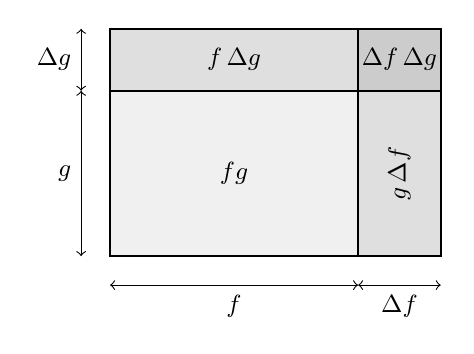
\begin{tikzpicture}[scale=1.05, every node/.style={font=\small}]
  % Dimensions
  \def\f{3.0}
  \def\g{2.0}
  \def\df{1.0}
  \def\dg{0.75}

  % Original rectangle
  \draw[fill=gray!12, thick] (0,0) rectangle (\f,\g);
  \node at (1.5,1.0) {\(fg\)};

  % Right strip
  \draw[fill=gray!25, thick] (\f,0) rectangle ({\f+\df},\g);
  \node[rotate=90] at ({\f+0.5*\df},1.0) {\(g\,\Delta f\)};

  % Top strip
  \draw[fill=gray!25, thick] (0,\g) rectangle (\f,{\g+\dg});
  \node at (1.5,{\g+0.38}) {\(f\,\Delta g\)};

  % Corner
  \draw[fill=gray!40, thick] (\f,\g) rectangle ({\f+\df},{\g+\dg});
  \node at ({\f+0.5*\df},{\g+0.38}) {\(\Delta f\,\Delta g\)};

  % Labels
  \draw[<->] (0,-0.35) -- (\f,-0.35);
  \node[below] at (1.5,-0.35) {\(f\)};

  \draw[<->] (\f,-0.35) -- ({\f+\df},-0.35);
  \node[below] at ({\f+0.5*\df},-0.35) {\(\Delta f\)};

  \draw[<->] (-0.35,0) -- (-0.35,\g);
  \node[left] at (-0.35,1.0) {\(g\)};

  \draw[<->] (-0.35,\g) -- (-0.35,{\g+\dg});
  \node[left] at (-0.35,{\g+0.5*\dg}) {\(\Delta g\)};
\end{tikzpicture}
\caption{When both factors change, a product changes by two main strips and a small corner.}
\label{fig:product-rule-area}
\end{figure}

Now divide by \(h\):

\[
\frac{\Delta(fg)}{h}
=
g\frac{\Delta f}{h}
+
f\frac{\Delta g}{h}
+
\Delta f\frac{\Delta g}{h}.
\]

As \(h\to0\),

\[
\frac{\Delta f}{h}\to f'(x),
\qquad
\frac{\Delta g}{h}\to g'(x).
\]

Also \(\Delta f\to0\), because differentiability implies continuity.  Therefore the last term

\[
\Delta f\frac{\Delta g}{h}
\]

approaches \(0\cdot g'(x)=0\).

The two main strips survive.  The tiny corner disappears in the limiting rate.

This gives the product rule.

\begin{quote}
\textbf{Product rule.}
If \(f\) and \(g\) are differentiable at \(x\), then

\[
\boxed{
\frac{d}{dx}\bigl(f(x)g(x)\bigr)
=
f'(x)g(x)+f(x)g'(x).
}
\]

In prime notation,

\[
\boxed{
(fg)'=f'g+fg'.
}
\]
\end{quote}

\paragraph{Proof.}
Let

\[
\Delta f=f(x+h)-f(x),
\qquad
\Delta g=g(x+h)-g(x).
\]

Then

\[
f(x+h)=f(x)+\Delta f
\]

and

\[
g(x+h)=g(x)+\Delta g.
\]

So

\[
f(x+h)g(x+h)-f(x)g(x)
=
g(x)\Delta f+f(x)\Delta g+\Delta f\,\Delta g.
\]

Divide by \(h\):

\[
\frac{f(x+h)g(x+h)-f(x)g(x)}{h}
=
g(x)\frac{\Delta f}{h}
+
f(x)\frac{\Delta g}{h}
+
\Delta f\frac{\Delta g}{h}.
\]

As \(h\to0\),

\[
\frac{\Delta f}{h}\to f'(x),
\]

\[
\frac{\Delta g}{h}\to g'(x),
\]

and

\[
\Delta f\to0.
\]

Therefore

\[
(fg)'(x)=g(x)f'(x)+f(x)g'(x).
\]

That is the product rule.

\paragraph{Differential form of the same idea.}
The exact change is

\[
\Delta(fg)=g\,\Delta f+f\,\Delta g+\Delta f\,\Delta g.
\]

The differential keeps only the linear part:

\[
\boxed{
d(fg)=g\,df+f\,dg.
}
\]

The corner term

\[
\Delta f\,\Delta g
\]

is a product of two small changes.  It is smaller than first order and is not part of the linear approximation.

\subsection{Using the product rule}
\label{subsec:using-product-rule}

\paragraph{Example.}
Differentiate

\[
F(x)=(x^2+1)(x^3-5).
\]

Let

\[
f(x)=x^2+1
\qquad\text{and}\qquad
g(x)=x^3-5.
\]

Then

\[
f'(x)=2x,
\qquad
g'(x)=3x^2.
\]

By the product rule,

\[
F'(x)=2x(x^3-5)+(x^2+1)(3x^2).
\]

Simplify:

\[
F'(x)=2x^4-10x+3x^4+3x^2.
\]

Thus

\[
\boxed{
F'(x)=5x^4+3x^2-10x.
}
\]

This matches what we would get by expanding first:

\[
(x^2+1)(x^3-5)=x^5+x^3-5x^2-5.
\]

But the product rule works even when expansion is not practical.

\paragraph{Example.}
Differentiate

\[
P(x)=x^4(x^2-3x+2).
\]

Here

\[
f(x)=x^4,
\qquad
g(x)=x^2-3x+2.
\]

Then

\[
f'(x)=4x^3,
\qquad
g'(x)=2x-3.
\]

So

\[
P'(x)=4x^3(x^2-3x+2)+x^4(2x-3).
\]

This is already a correct derivative.  If desired, simplify:

\[
P'(x)=4x^5-12x^4+8x^3+2x^5-3x^4,
\]

so

\[
\boxed{
P'(x)=6x^5-15x^4+8x^3.
}
\]

\paragraph{Warning: \((fg)'\neq f'g'\).}
Take

\[
f(x)=x,
\qquad
g(x)=x.
\]

Then

\[
f(x)g(x)=x^2,
\]

so

\[
(fg)'=2x.
\]

But

\[
f'(x)g'(x)=1\cdot1=1.
\]

These are not the same function.

The product rule says

\[
(fg)'=f'g+fg',
\]

not

\[
(fg)'=f'g'.
\]

\paragraph{A hypothesis warning.}
The product rule says that if both factors are differentiable, then the product is differentiable.  The converse is not true.

Let

\[
F(x)=x|x|.
\]

The factor \(|x|\) is not differentiable at \(0\), so the product rule cannot be used at \(0\).  But \(F\) itself is differentiable at \(0\).  Indeed,

\[
F'(0)
=
\lim_{h\to0}\frac{h|h|-0}{h}
=
\lim_{h\to0}|h|
=
0.
\]

So a product may have a derivative even when one factor does not.  The rule gives a safe sufficient condition, not a complete test for every possible product.

\subsection{The reciprocal rule}
\label{subsec:reciprocal-rule}

Quotients begin with reciprocals.  If

\[
u(x)=\frac1{g(x)},
\]

then \(u\) changes in the opposite direction from \(g\).  When the denominator increases, the reciprocal decreases.

The derivative formula is:

\[
\boxed{
\frac{d}{dx}\left(\frac1{g(x)}\right)
=
-\frac{g'(x)}{(g(x))^2},
}
\]

where \(g(x)\neq0\).

\paragraph{Proof.}
Let

\[
u(x)=\frac1{g(x)}.
\]

Then

\[
u'(x)
=
\lim_{h\to0}
\frac{\frac1{g(x+h)}-\frac1{g(x)}}{h}.
\]

Combine the fractions:

\[
\frac{\frac1{g(x+h)}-\frac1{g(x)}}{h}
=
\frac{g(x)-g(x+h)}{h\,g(x+h)g(x)}.
\]

Rewrite the numerator:

\[
g(x)-g(x+h)=-(g(x+h)-g(x)).
\]

So

\[
\frac{\frac1{g(x+h)}-\frac1{g(x)}}{h}
=
-\frac{g(x+h)-g(x)}{h\,g(x+h)g(x)}.
\]

Now let \(h\to0\).  Since \(g\) is differentiable, it is continuous.  Therefore

\[
g(x+h)\to g(x).
\]

Also,

\[
\frac{g(x+h)-g(x)}{h}\to g'(x).
\]

Thus

\[
u'(x)
=
-\frac{g'(x)}{g(x)^2}.
\]

\paragraph{Example.}
Differentiate

\[
R(x)=\frac1{x^2+1}.
\]

Let

\[
g(x)=x^2+1.
\]

Then

\[
g'(x)=2x.
\]

By the reciprocal rule,

\[
R'(x)
=
-\frac{2x}{(x^2+1)^2}.
\]

So

\[
\boxed{
\frac{d}{dx}\left(\frac1{x^2+1}\right)
=
-\frac{2x}{(x^2+1)^2}.
}
\]

\paragraph{Negative powers.}
The reciprocal rule also extends the power rule to negative integer powers.

For \(n\) a positive integer,

\[
x^{-n}=\frac1{x^n},
\qquad x\neq0.
\]

Using the reciprocal rule with

\[
g(x)=x^n,
\]

we get

\[
\frac{d}{dx}x^{-n}
=
-\frac{nx^{n-1}}{(x^n)^2}.
\]

Since

\[
(x^n)^2=x^{2n},
\]

this becomes

\[
-nx^{n-1-2n}
=
-nx^{-n-1}.
\]

So

\[
\boxed{
\frac{d}{dx}x^{-n}=-n x^{-n-1}
\qquad (x\neq0).
}
\]

This is the same pattern as the power rule:

\[
\frac{d}{dx}x^r=rx^{r-1}.
\]

We have now proved it for positive and negative integer powers.  Fractional powers will come later.

\subsection{The quotient rule}
\label{subsec:quotient-rule}

A quotient is a product with a reciprocal:

\[
\frac{f(x)}{g(x)}
=
f(x)\cdot\frac1{g(x)}.
\]

So the quotient rule follows from the product rule and the reciprocal rule.

\begin{quote}
\textbf{Quotient rule.}
If \(f\) and \(g\) are differentiable at \(x\), and \(g(x)\neq0\), then

\[
\boxed{
\frac{d}{dx}\left(\frac{f(x)}{g(x)}\right)
=
\frac{g(x)f'(x)-f(x)g'(x)}{(g(x))^2}.
}
\]
\end{quote}

\paragraph{Derivation.}
Write

\[
\frac{f}{g}=f\cdot\frac1g.
\]

Then

\[
\left(\frac{f}{g}\right)'
=
f'\cdot\frac1g
+
f\cdot\left(\frac1g\right)'.
\]

Using the reciprocal rule,

\[
\left(\frac1g\right)'=-\frac{g'}{g^2}.
\]

Therefore

\[
\left(\frac{f}{g}\right)'
=
\frac{f'}{g}
-
\frac{fg'}{g^2}.
\]

Put both terms over the common denominator \(g^2\):

\[
\left(\frac{f}{g}\right)'
=
\frac{gf'-fg'}{g^2}.
\]

\paragraph{Example.}
Differentiate

\[
Q(x)=\frac{x^2+1}{x-3}.
\]

Let

\[
f(x)=x^2+1,
\qquad
g(x)=x-3.
\]

Then

\[
f'(x)=2x,
\qquad
g'(x)=1.
\]

The quotient rule gives

\[
Q'(x)
=
\frac{(x-3)(2x)-(x^2+1)(1)}{(x-3)^2}.
\]

Simplify the numerator:

\[
(x-3)(2x)-(x^2+1)
=
2x^2-6x-x^2-1
=
x^2-6x-1.
\]

Thus

\[
\boxed{
Q'(x)=\frac{x^2-6x-1}{(x-3)^2}
}
\]

for

\[
x\neq3.
\]

\paragraph{Example.}
Differentiate

\[
R(x)=\frac{x^3}{x^2+1}.
\]

Let

\[
f(x)=x^3,
\qquad
g(x)=x^2+1.
\]

Then

\[
f'(x)=3x^2,
\qquad
g'(x)=2x.
\]

So

\[
R'(x)
=
\frac{(x^2+1)(3x^2)-x^3(2x)}{(x^2+1)^2}.
\]

Simplify:

\[
R'(x)
=
\frac{3x^4+3x^2-2x^4}{(x^2+1)^2}
=
\frac{x^4+3x^2}{(x^2+1)^2}.
\]

Therefore

\[
\boxed{
R'(x)=\frac{x^4+3x^2}{(x^2+1)^2}.
}
\]

\subsection{When a denominator erases a point}
\label{subsec:denominator-erases-point}

The quotient rule requires

\[
g(x)\neq0.
\]

This matters.

Consider

\[
H(x)=\frac{x^2-1}{x-1}.
\]

For \(x\neq1\), we can factor:

\[
H(x)=\frac{(x-1)(x+1)}{x-1}=x+1.
\]

So for \(x\neq1\),

\[
H'(x)=1.
\]

But the original function \(H\) is not defined at \(x=1\).  Therefore \(H'(1)\) does not exist.  A function cannot have a derivative at a point where it is not defined.

If we fill the hole by defining a new function

\[
\widetilde H(x)=
\begin{cases}
\dfrac{x^2-1}{x-1}, & x\neq1,\\[8pt]
2, & x=1,
\end{cases}
\]

then

\[
\widetilde H(x)=x+1
\]

for every \(x\), including \(x=1\).  In that new case,

\[
\widetilde H'(1)=1.
\]

\begin{quote}
\textbf{A quotient rule warning.}
Simplifying a quotient can reveal nearby behavior, but it does not automatically define the missing point.  Differentiability at a point requires the function to exist at that point.
\end{quote}

\subsection{The rules so far}
\label{subsec:rules-so-far}

We now have a larger toolbox:

\[
\frac{d}{dx}(c)=0,
\]

\[
\frac{d}{dx}x^n=nx^{n-1}
\qquad(n=1,2,3,\ldots),
\]

\[
\frac{d}{dx}\bigl(a f+b g\bigr)=a f'+b g',
\]

\[
\frac{d}{dx}(fg)=f'g+fg',
\]

\[
\frac{d}{dx}\left(\frac1g\right)=-\frac{g'}{g^2},
\]

and

\[
\frac{d}{dx}\left(\frac{f}{g}\right)=\frac{gf'-fg'}{g^2}.
\]

These rules handle many expressions built by adding, scaling, multiplying, and dividing.

But one common construction is still missing.  Many functions are nested:

\[
(x^2+1)^5,
\qquad
\sqrt{x^3+1},
\qquad
\frac1{(2x-7)^4}.
\]

The outside function changes because the inside function changes first.  The next rule measures change through a chain.
\section{The chain rule}
\label{sec:chain-rule}

The product rule handled functions built side by side:

\[
f(x)g(x).
\]

Composition is more hidden.  One function changes because another function inside it changes first:

\[
f(g(x)).
\]

This happens constantly.  A temperature changes because position changes.  A cost changes because production changes.  A population changes because time changes.  The outside quantity does not see \(x\) directly.  It sees an intermediate quantity.

\subsection{A temperature that changes because position changes}
\label{subsec:temperature-position-chain}

A small sensor moves along a wire.  Its position after \(t\) seconds is

\[
x(t)=t^2
\]

centimeters from one end of the wire.  The temperature at position \(x\) is

\[
T(x)=100-x^2
\]

degrees Celsius.

At time \(t\), the sensor reads the temperature

\[
T(x(t)).
\]

Since \(x(t)=t^2\), this is

\[
T(x(t))=T(t^2)=100-(t^2)^2=100-t^4.
\]

So we can differentiate directly:

\[
\frac{d}{dt}T(x(t))
=
\frac{d}{dt}(100-t^4)
=
-4t^3.
\]

At \(t=2\),

\[
\frac{d}{dt}T(x(t))\bigg|_{t=2}
=
-4(2)^3
=
-32.
\]

The sensor's reading is decreasing at \(32\) degrees Celsius per second.

But the direct calculation hides the reason.  Two changes are happening:

\[
t \longrightarrow x \longrightarrow T.
\]

The position changes with respect to time:

\[
\frac{dx}{dt}=2t.
\]

The temperature changes with respect to position:

\[
\frac{dT}{dx}=-2x.
\]

At \(t=2\), the sensor is at

\[
x(2)=4.
\]

So

\[
\frac{dT}{dx}\bigg|_{x=4}=-8,
\qquad
\frac{dx}{dt}\bigg|_{t=2}=4.
\]

Multiplying gives

\[
\frac{dT}{dt}
=
\frac{dT}{dx}\frac{dx}{dt}
=
(-8)(4)
=
-32.
\]

The same answer appears, but now we see why it is a product:

\[
\boxed{
\begin{aligned}
&\text{rate of temperature change in time} \\
&\quad = \text{rate of temperature change in space} \\
&\quad\quad \cdot \text{rate of position change in time}.
\end{aligned}
}
\]

The outside change is carried through the inside change.

\subsection{Composition as change inside change}
\label{subsec:composition-change-inside-change}

A composition has the form

\[
y=f(g(x)).
\]

It is often clearer to name the inside quantity:

\[
u=g(x),
\qquad
y=f(u).
\]

Then the dependence is

\[
x \longrightarrow u \longrightarrow y.
\]

A small change in \(x\) first causes a small change in \(u\).  Then that small change in \(u\) causes a small change in \(y\).

If \(u\) changes at the rate \(du/dx\), and \(y\) changes at the rate \(dy/du\), then we expect

\[
\frac{dy}{dx}
=
\frac{dy}{du}\frac{du}{dx}.
\]

This is the chain rule.

Before stating it in full, try it on a function we could differentiate by expanding, but do not want to.

\paragraph{Example.}
Differentiate

\[
y=(x^2+1)^5.
\]

The inside function is

\[
u=x^2+1.
\]

The outside function is

\[
y=u^5.
\]

The outside rate is

\[
\frac{dy}{du}=5u^4.
\]

The inside rate is

\[
\frac{du}{dx}=2x.
\]

Therefore

\[
\frac{dy}{dx}
=
5u^4\cdot 2x.
\]

Substitute back \(u=x^2+1\):

\[
\boxed{
\frac{d}{dx}(x^2+1)^5
=
10x(x^2+1)^4.
}
\]

Expanding \((x^2+1)^5\) would work, but it would make a simple idea look complicated.  The chain rule keeps the structure visible.

\subsection{The chain rule formula}
\label{subsec:chain-rule-formula}

\begin{quote}
\textbf{Chain Rule.}
Suppose \(g\) is differentiable at \(x\), and \(f\) is differentiable at \(g(x)\).  Then the composite function

\[
F(x)=f(g(x))
\]

is differentiable at \(x\), and

\[
\boxed{
F'(x)=f'(g(x))\,g'(x).
}
\]

Equivalently, if

\[
u=g(x),
\qquad
y=f(u),
\]

then

\[
\boxed{
\frac{dy}{dx}
=
\frac{dy}{du}\frac{du}{dx}.
}
\]
\end{quote}

The formula has two factors:

\[
f'(g(x))
\]

measures how the outside function changes at the current inside value, and

\[
g'(x)
\]

measures how the inside function changes with respect to \(x\).

\paragraph{Example.}
Differentiate

\[
F(x)=(3x^2-5x+1)^4.
\]

Let

\[
u=3x^2-5x+1.
\]

Then

\[
F(x)=u^4.
\]

The outside derivative is

\[
\frac{d}{du}(u^4)=4u^3.
\]

The inside derivative is

\[
\frac{du}{dx}=6x-5.
\]

Thus

\[
F'(x)=4u^3(6x-5).
\]

Substitute back:

\[
\boxed{
F'(x)
=
4(3x^2-5x+1)^3(6x-5).
}
\]

\paragraph{Example.}
Differentiate

\[
G(x)=\frac{1}{1+x^2}.
\]

This can be seen as a reciprocal wrapped around the inside function

\[
u=1+x^2.
\]

The outside function is

\[
G=\frac1u.
\]

The reciprocal rule gives

\[
\frac{d}{du}\left(\frac1u\right)=-\frac1{u^2}.
\]

The inside derivative is

\[
\frac{du}{dx}=2x.
\]

Therefore

\[
G'(x)
=
-\frac1{u^2}\cdot 2x
=
-\frac{2x}{(1+x^2)^2}.
\]

So

\[
\boxed{
\frac{d}{dx}\left(\frac{1}{1+x^2}\right)
=
-\frac{2x}{(1+x^2)^2}.
}
\]

\paragraph{Example.}
Differentiate

\[
H(x)=\frac{1}{(1+x^2)^3}.
\]

We could think of this as a reciprocal:

\[
H(x)=\frac1{W(x)},
\qquad
W(x)=(1+x^2)^3.
\]

First use the chain rule on \(W\).  Let

\[
u=1+x^2.
\]

Then

\[
W=u^3,
\]

so

\[
W'(x)=3u^2\cdot 2x=6x(1+x^2)^2.
\]

Now use the reciprocal rule:

\[
H'(x)
=
-\frac{W'(x)}{W(x)^2}.
\]

Thus

\[
H'(x)
=
-\frac{6x(1+x^2)^2}{\bigl((1+x^2)^3\bigr)^2}.
\]

Since

\[
\bigl((1+x^2)^3\bigr)^2=(1+x^2)^6,
\]

we get

\[
\boxed{
H'(x)
=
-\frac{6x}{(1+x^2)^4}.
}
\]

The chain rule often works together with earlier rules.  The expression is built in layers, and the derivative follows those layers.

\subsection{Why the chain rule is true}
\label{subsec:why-chain-rule-true}

The derivative is local linear approximation.  That idea explains the chain rule better than symbol cancellation alone.

Suppose

\[
u=g(x),
\qquad
y=f(u).
\]

Near a point \(x=a\), the inside function satisfies

\[
g(a+h)\approx g(a)+g'(a)h.
\]

So the inside change is approximately

\[
\Delta u \approx g'(a)h.
\]

Near \(u=g(a)\), the outside function satisfies

\[
f(u+\Delta u)\approx f(u)+f'(u)\Delta u.
\]

Thus the outside change is approximately

\[
\Delta y \approx f'(u)\Delta u.
\]

Substitute the inside change:

\[
\Delta y
\approx
f'(g(a))\bigl(g'(a)h\bigr).
\]

Divide by \(h\):

\[
\frac{\Delta y}{h}
\approx
f'(g(a))g'(a).
\]

Letting \(h\to0\) gives

\[
\frac{d}{dx}f(g(x))\bigg|_{x=a}
=
f'(g(a))g'(a).
\]

\paragraph{Proof.}
Let

\[
u_0=g(a).
\]

Since \(f\) is differentiable at \(u_0\), we can write its local linear approximation with an error term:

\[
f(u_0+k)
=
f(u_0)+f'(u_0)k+k\varepsilon(k),
\]

where

\[
\varepsilon(k)\to0
\qquad\text{as}\qquad
k\to0.
\]

Now put

\[
k=g(a+h)-g(a).
\]

Then

\[
f(g(a+h))
=
f(g(a))+f'(g(a))\bigl(g(a+h)-g(a)\bigr)
+
\bigl(g(a+h)-g(a)\bigr)\varepsilon(k).
\]

Subtract \(f(g(a))\) and divide by \(h\):

\[
\frac{f(g(a+h))-f(g(a))}{h}
=
f'(g(a))\frac{g(a+h)-g(a)}{h}
+
\frac{g(a+h)-g(a)}{h}\varepsilon(k).
\]

Because \(g\) is differentiable at \(a\),

\[
\frac{g(a+h)-g(a)}{h}\to g'(a).
\]

Also, differentiability of \(g\) implies continuity of \(g\), so

\[
g(a+h)-g(a)\to0.
\]

Thus \(k\to0\), and therefore

\[
\varepsilon(k)\to0.
\]

Taking limits gives

\[
(f\circ g)'(a)
=
f'(g(a))g'(a)+g'(a)\cdot0.
\]

Hence

\[
\boxed{
(f\circ g)'(a)=f'(g(a))g'(a).
}
\]

This proves the chain rule.

\subsection{Why the hypotheses are there}
\label{subsec:chain-rule-hypotheses}

The chain rule assumes that the inside function is differentiable at the point, and that the outside function is differentiable at the inside value.  Both assumptions matter.

\paragraph{The outside function must be differentiable at the inside value.}
Let

\[
f(u)=|u|,
\qquad
g(x)=x.
\]

Then

\[
f(g(x))=|x|.
\]

At \(x=0\), the inside value is

\[
g(0)=0.
\]

But \(f(u)=|u|\) is not differentiable at \(u=0\).  The composite \(|x|\) is not differentiable at \(x=0\).  There is no chain rule product to compute there.

\paragraph{The inside function must be differentiable at the point.}
Let

\[
f(u)=u,
\qquad
g(x)=|x|.
\]

Then

\[
f(g(x))=|x|.
\]

The outside function \(f(u)=u\) is differentiable everywhere, but \(g(x)=|x|\) is not differentiable at \(x=0\).  Again the composite is not differentiable at \(0\).

\begin{quote}
\textbf{Moral.}
A composite function can only inherit a derivative through the chain rule when both links in the chain have derivatives at the needed places.
\end{quote}

\subsection{Tree diagrams for nested functions}
\label{subsec:tree-diagrams-chain-rule}

When a formula has several layers, a diagram can prevent mistakes.

Consider

\[
y=\left(1+(2x-3)^2\right)^5.
\]

The layers are

\[
x \longrightarrow u=2x-3 \longrightarrow v=1+u^2 \longrightarrow y=v^5.
\]

\begin{figure}[h]
\centering
\begin{tikzpicture}[node distance=2.4cm, every node/.style={font=\small}]
  \node (x) at (0,0) {\(\boxed{x}\)};
  \node (u) at (2.6,0) {\(\boxed{u=2x-3}\)};
  \node (v) at (5.4,0) {\(\boxed{v=1+u^2}\)};
  \node (y) at (8.2,0) {\(\boxed{y=v^5}\)};

  \draw[->, thick] (x) -- (u);
  \draw[->, thick] (u) -- (v);
  \draw[->, thick] (v) -- (y);

  \node[above] at (1.3,0.25) {\(\dfrac{du}{dx}=2\)};
  \node[above] at (4.0,0.25) {\(\dfrac{dv}{du}=2u\)};
  \node[above] at (6.8,0.25) {\(\dfrac{dy}{dv}=5v^4\)};
\end{tikzpicture}
\caption{A chain diagram records the order in which the function is built.}
\label{fig:chain-diagram}
\end{figure}

The derivative is the product of the derivatives along the chain:

\[
\frac{dy}{dx}
=
\frac{dy}{dv}\frac{dv}{du}\frac{du}{dx}.
\]

So

\[
\frac{dy}{dx}
=
5v^4\cdot 2u\cdot 2.
\]

Substitute back:

\[
u=2x-3,
\qquad
v=1+(2x-3)^2.
\]

Therefore

\[
\boxed{
\frac{d}{dx}\left(1+(2x-3)^2\right)^5
=
20(2x-3)\left(1+(2x-3)^2\right)^4.
}
\]

Some expressions branch before they recombine.  Then the product rule and chain rule work together.

\paragraph{Example.}
Differentiate

\[
y=\bigl((x^2+1)(3x-2)\bigr)^4.
\]

Let

\[
v=x^2+1,
\qquad
w=3x-2,
\qquad
u=vw,
\qquad
y=u^4.
\]

The outside derivative is

\[
\frac{dy}{du}=4u^3.
\]

The derivative of \(u=vw\) is

\[
\frac{du}{dx}=v'w+vw'.
\]

Here

\[
v'=2x,
\qquad
w'=3.
\]

So

\[
u'=2x(3x-2)+3(x^2+1).
\]

Therefore

\[
\boxed{
y'
=
4\bigl((x^2+1)(3x-2)\bigr)^3
\left(2x(3x-2)+3(x^2+1)\right).
}
\]

The outside power contributes the factor

\[
4u^3.
\]

The inside product contributes the factor

\[
u'=v'w+vw'.
\]

A diagram is not required, but it helps keep the structure from collapsing into a long line of symbols.

\subsection{The order of composition matters}
\label{subsec:composition-order-warning}

Composition is not commutative.  Usually,

\[
f(g(x))\neq g(f(x)).
\]

The derivatives are also different.

\paragraph{Example.}
Let

\[
f(u)=u^2,
\qquad
g(x)=x+1.
\]

Then

\[
f(g(x))=(x+1)^2,
\]

so

\[
\frac{d}{dx}f(g(x))=2(x+1).
\]

But

\[
g(f(x))=x^2+1,
\]

so

\[
\frac{d}{dx}g(f(x))=2x.
\]

The same two functions, used in a different order, produce different composites.

\begin{quote}
\textbf{Chain rule warning.}
Differentiate from the outside inward, but preserve the order in which the function is built.
\end{quote}

\subsection{Chain rule in differential notation}
\label{subsec:chain-rule-differential-notation}

The notation

\[
\frac{dy}{dx}
=
\frac{dy}{du}\frac{du}{dx}
\]

looks like canceling \(du\).  That is a useful memory, but it is not the proof.  The proof came from local linear approximation.

The notation is still meaningful.  If

\[
y=f(u),
\]

then a small change in \(u\) produces

\[
dy=f'(u)\,du.
\]

If

\[
u=g(x),
\]

then a small change in \(x\) produces

\[
du=g'(x)\,dx.
\]

Substitute the second relation into the first:

\[
dy=f'(u)g'(x)\,dx.
\]

Since \(u=g(x)\),

\[
dy=f'(g(x))g'(x)\,dx.
\]

Dividing by \(dx\) gives

\[
\frac{dy}{dx}=f'(g(x))g'(x).
\]

This is the same chain rule.

The differential notation remembers the units.  In the temperature example,

\[
\frac{dT}{dx}
\]

has units degrees per centimeter, and

\[
\frac{dx}{dt}
\]

has units centimeters per second.  Their product has units

\[
\frac{\text{degrees}}{\text{centimeter}}
\cdot
\frac{\text{centimeters}}{\text{second}}
=
\frac{\text{degrees}}{\text{second}}.
\]

That is exactly the unit of

\[
\frac{dT}{dt}.
\]

The chain rule lets us differentiate functions built in layers.  It also gives a way to handle curves whose equations are not solved for \(y\).  On such a curve, \(y\) changes because \(x\) changes, even when no formula \(y=f(x)\) has been written down.

\section{Implicit differentiation}
\label{sec:implicit-differentiation}

Many curves are not naturally written as

\[
y=f(x).
\]

A circle is easier to describe by

\[
x^2+y^2=25
\]

than by two separate formulas

\[
y=\sqrt{25-x^2}
\qquad\text{and}\qquad
y=-\sqrt{25-x^2}.
\]

The equation relates \(x\) and \(y\) without solving for \(y\).  Such an equation defines a curve \emph{implicitly}.

The chain rule lets us find slopes on these curves directly.

\subsection{Curves not solved for \(y\)}
\label{subsec:curves-not-solved-for-y}

The equation

\[
x^2+y^2=25
\]

does not describe one function \(y=f(x)\) on the whole circle.  Most vertical lines through the circle meet it twice: once on the upper half and once on the lower half.

But near the point

\[
(3,4),
\]

the upper half of the circle can be treated as a function of \(x\).  As \(x\) changes a little, \(y\) changes in a definite way to keep the point on the circle.

We want the slope

\[
\frac{dy}{dx}
\]

at \((3,4)\).

Solving for \(y\) is possible here:

\[
y=\sqrt{25-x^2}
\]

on the upper half.  But differentiating the original equation is cleaner and teaches a method that works even when solving for \(y\) is unpleasant.

Start with

\[
x^2+y^2=25.
\]

Think of \(y\) as a function of \(x\), even though we have not written its formula.  Differentiate both sides with respect to \(x\).

The derivative of \(x^2\) is

\[
2x.
\]

The derivative of \(y^2\) is not simply \(2y\).  Since \(y\) depends on \(x\), the chain rule gives

\[
\frac{d}{dx}(y^2)=2y\frac{dy}{dx}.
\]

The derivative of \(25\) is \(0\).  Therefore

\[
2x+2y\frac{dy}{dx}=0.
\]

Solve for \(dy/dx\):

\[
2y\frac{dy}{dx}=-2x,
\]

so

\[
\boxed{
\frac{dy}{dx}=-\frac{x}{y}.
}
\]

At \((3,4)\),

\[
\frac{dy}{dx}
=
-\frac34.
\]

So the tangent line has slope \(-3/4\).

\begin{figure}[h]
\centering
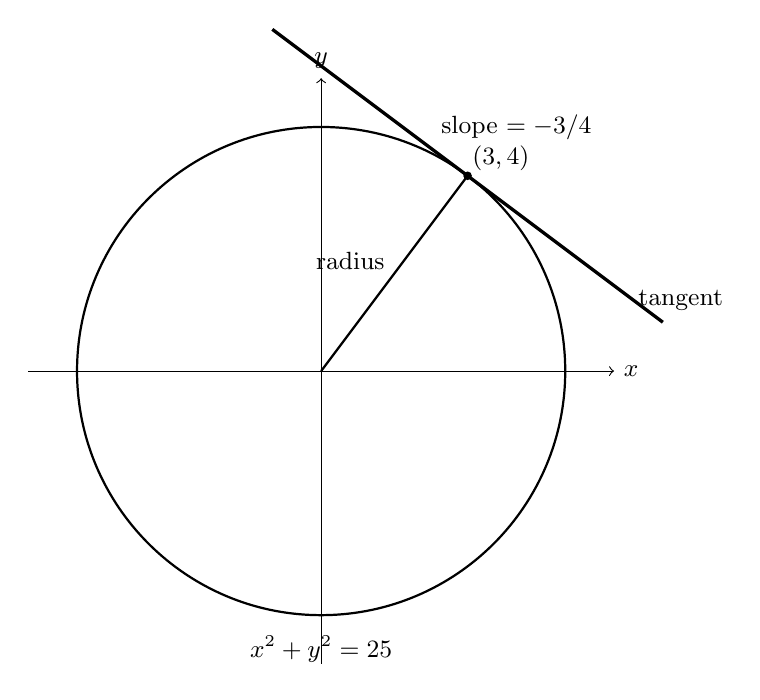
\begin{tikzpicture}[scale=0.62, every node/.style={font=\small}]
  % axes
  \draw[->] (-6,0) -- (6,0) node[right] {\(x\)};
  \draw[->] (0,-6) -- (0,6) node[above] {\(y\)};

  % circle
  \draw[thick] (0,0) circle (5);

  % point (3,4)
  \fill (3,4) circle (2.5pt);
  \node[above right] at (2.9,3.9) {\((3,4)\)};

  % radius
  \draw[thick] (0,0) -- (3,4);
  \node[left] at (1.5,2.25) {radius};

  % tangent line slope -3/4, direction (4,-3)
  \draw[very thick] (-1,7) -- (7,1);
  \node[right] at (6.3,1.45) {tangent};

  % slope note
  \node at (0,-5.7) {\(x^2+y^2=25\)};
  \node at (4.0,5.0) {slope \(=-3/4\)};
\end{tikzpicture}
\caption{Implicit differentiation gives the tangent slope without solving the circle into upper and lower functions.}
\label{fig:circle-implicit-tangent}
\end{figure}

The tangent line at \((3,4)\) is

\[
y-4=-\frac34(x-3).
\]

Equivalently,

\[
3x+4y=25.
\]

This matches the geometry: the radius from \((0,0)\) to \((3,4)\) has slope \(4/3\), and the tangent has the negative reciprocal slope \(-3/4\).  The radius and tangent are perpendicular.

\subsection{Differentiating both sides}
\label{subsec:differentiating-both-sides-implicit}

The circle example used the main rule of implicit differentiation.

\begin{quote}
\textbf{Implicit differentiation.}
When an equation relates \(x\) and \(y\), and \(y\) is treated as a differentiable function of \(x\), differentiate both sides with respect to \(x\).  Every time a derivative falls on \(y\), use the chain rule.

For example,

\[
\frac{d}{dx}(y^n)
=
ny^{n-1}\frac{dy}{dx}.
\]
\end{quote}

The notation is often shortened by writing

\[
y'=\frac{dy}{dx}.
\]

Then

\[
\frac{d}{dx}(y^2)=2yy',
\]

and

\[
\frac{d}{dx}(y^5)=5y^4y'.
\]

\paragraph{Example.}
Find \(dy/dx\) if

\[
y^3+xy=10.
\]

Differentiate both sides with respect to \(x\).

The derivative of \(y^3\) is

\[
3y^2y'.
\]

The derivative of \(xy\) uses the product rule:

\[
\frac{d}{dx}(xy)=x y'+y.
\]

The derivative of \(10\) is \(0\).  Therefore

\[
3y^2y'+xy'+y=0.
\]

Collect the terms containing \(y'\):

\[
(3y^2+x)y'+y=0.
\]

So

\[
(3y^2+x)y'=-y,
\]

and

\[
\boxed{
\frac{dy}{dx}
=
-\frac{y}{3y^2+x}.
}
\]

At the point \((1,2)\), the equation is satisfied because

\[
2^3+1\cdot2=8+2=10.
\]

The slope there is

\[
\frac{dy}{dx}\bigg|_{(1,2)}
=
-\frac{2}{3(2)^2+1}
=
-\frac{2}{13}.
\]

So the tangent line at \((1,2)\) is

\[
y-2=-\frac{2}{13}(x-1).
\]

\paragraph{Example.}
Find \(dy/dx\) for

\[
x^2+xy+y^2=7.
\]

Differentiate both sides:

\[
\frac{d}{dx}(x^2)
+
\frac{d}{dx}(xy)
+
\frac{d}{dx}(y^2)
=
\frac{d}{dx}(7).
\]

This gives

\[
2x+(xy'+y)+2yy'=0.
\]

Collect \(y'\)-terms:

\[
xy'+2yy'+2x+y=0.
\]

So

\[
(x+2y)y'=-(2x+y).
\]

Therefore

\[
\boxed{
\frac{dy}{dx}
=
-\frac{2x+y}{x+2y}.
}
\]

At \((1,2)\), the equation is satisfied:

\[
1^2+1\cdot2+2^2=1+2+4=7.
\]

The slope is

\[
\frac{dy}{dx}\bigg|_{(1,2)}
=
-\frac{2(1)+2}{1+2(2)}
=
-\frac45.
\]

The tangent line is

\[
y-2=-\frac45(x-1).
\]

\subsection{The chain rule is doing the hidden work}
\label{subsec:hidden-chain-rule-implicit}

Implicit differentiation can feel like a new trick, but it is only the chain rule applied carefully.

Suppose

\[
y=y(x).
\]

Then

\[
y^3
\]

is really the composite function

\[
(y(x))^3.
\]

By the chain rule,

\[
\frac{d}{dx}(y(x))^3
=
3(y(x))^2y'(x).
\]

In shortened notation,

\[
\frac{d}{dx}(y^3)=3y^2y'.
\]

The same pattern gives

\[
\frac{d}{dx}(5y^4)=20y^3y',
\]

and

\[
\frac{d}{dx}(x^2y^3)
=
2xy^3+x^2(3y^2y').
\]

The first term comes from differentiating \(x^2\).  The second term comes from differentiating \(y^3\), which requires the chain rule.

\paragraph{Example.}
Differentiate

\[
x^2y^3+y=4x.
\]

The derivative of \(x^2y^3\) uses the product rule:

\[
\frac{d}{dx}(x^2y^3)
=
2xy^3+x^2(3y^2y').
\]

The derivative of \(y\) is \(y'\).  The derivative of \(4x\) is \(4\).  Therefore

\[
2xy^3+3x^2y^2y'+y'=4.
\]

Collect \(y'\)-terms:

\[
(3x^2y^2+1)y'=4-2xy^3.
\]

So

\[
\boxed{
\frac{dy}{dx}
=
\frac{4-2xy^3}{3x^2y^2+1}.
}
\]

Every occurrence of \(y\) is a reminder that \(y\) depends on \(x\).

\subsection{When the method warns us}
\label{subsec:implicit-method-warnings}

Implicit differentiation assumes that near the point we care about, the curve can be treated as one differentiable function \(y(x)\).  The equation itself does not always guarantee that.

\paragraph{A vertical tangent.}
Consider the circle

\[
x^2+y^2=25
\]

at the point \((5,0)\).  Differentiating gives

\[
2x+2yy'=0.
\]

At \((5,0)\), this becomes

\[
10+0\cdot y'=0.
\]

No finite value of \(y'\) can satisfy this equation.  That does not mean the circle has no tangent.  It means the tangent is vertical, so its slope \(dy/dx\) is not a finite number.

The point \((5,0)\) is also where the upper and lower branches meet at the right edge.  Near that point, the circle cannot be written as a differentiable function \(y(x)\) with a finite derivative.

\paragraph{A relation with two branches.}
The equation

\[
y^2=x^2
\]

describes two lines:

\[
y=x
\qquad\text{and}\qquad
y=-x.
\]

At \((0,0)\), both branches meet.  If we choose the branch \(y=x\), the slope is \(1\).  If we choose the branch \(y=-x\), the slope is \(-1\).

Implicit differentiation gives

\[
2yy'=2x,
\]

or

\[
yy'=x.
\]

At \((0,0)\), this becomes

\[
0=0,
\]

which does not determine \(y'\).  The reason is geometric: the equation has not selected one branch.

\begin{quote}
\textbf{Implicit differentiation warning.}
When the equation does not define one smooth branch \(y(x)\) near the point, the algebra may produce no slope, many possible slopes, or an equation that does not determine \(dy/dx\).
\end{quote}

These warnings are useful.  They do not break the method.  They tell us what the geometry is doing.

\subsection{Higher derivatives implicitly}
\label{subsec:higher-derivatives-implicit}

Implicit differentiation can be repeated.  The main rule is the same: every time we differentiate an expression involving \(y\), remember that \(y\) depends on \(x\).

Return to the circle

\[
x^2+y^2=25.
\]

We found

\[
y'=-\frac{x}{y}.
\]

To find the second derivative, differentiate again:

\[
y''=\frac{d}{dx}\left(-\frac{x}{y}\right).
\]

Use the quotient rule on

\[
-\frac{x}{y}.
\]

First,

\[
\frac{d}{dx}\left(\frac{x}{y}\right)
=
\frac{y\cdot 1-x y'}{y^2}
=
\frac{y-xy'}{y^2}.
\]

Therefore

\[
y''
=
-\frac{y-xy'}{y^2}.
\]

Now substitute

\[
y'=-\frac{x}{y}.
\]

Then

\[
y-xy'
=
y-x\left(-\frac{x}{y}\right)
=
y+\frac{x^2}{y}.
\]

So

\[
y''
=
-\frac{y+\frac{x^2}{y}}{y^2}.
\]

Combine the numerator:

\[
y+\frac{x^2}{y}
=
\frac{y^2+x^2}{y}.
\]

Thus

\[
y''
=
-\frac{x^2+y^2}{y^3}.
\]

On the circle,

\[
x^2+y^2=25,
\]

so

\[
\boxed{
y''=-\frac{25}{y^3}.
}
\]

At \((3,4)\),

\[
y''=-\frac{25}{4^3}=-\frac{25}{64}.
\]

The negative sign says that the upper half of the circle is concave down at \((3,4)\).

\paragraph{Example.}
Find \(y''\) for

\[
y^3+xy=10.
\]

First derivative:

\[
3y^2y'+xy'+y=0.
\]

Differentiate again.  For \(3y^2y'\), use the product rule:

\[
\frac{d}{dx}(3y^2y')
=
3\left(2yy'\cdot y' + y^2y''\right)
=
6y(y')^2+3y^2y''.
\]

For \(xy'\), use the product rule:

\[
\frac{d}{dx}(xy')=xy''+y'.
\]

For \(y\), the derivative is \(y'\).  Therefore

\[
6y(y')^2+3y^2y''+xy''+y'+y'=0.
\]

Collect \(y''\)-terms:

\[
(3y^2+x)y''+6y(y')^2+2y'=0.
\]

So

\[
\boxed{
y''
=
-\frac{6y(y')^2+2y'}{3y^2+x}.
}
\]

This formula still contains \(y'\).  That is acceptable, but if we want \(y''\) in terms of \(x\) and \(y\) alone, we substitute

\[
y'=-\frac{y}{3y^2+x}.
\]

At \((1,2)\), we already found

\[
y'=-\frac{2}{13}.
\]

Therefore

\[
y''
=
-\frac{6(2)\left(-\frac{2}{13}\right)^2+2\left(-\frac{2}{13}\right)}{3(2)^2+1}.
\]

Compute the numerator:

\[
6(2)\left(\frac{4}{169}\right)-\frac{4}{13}
=
\frac{48}{169}-\frac{52}{169}
=
-\frac{4}{169}.
\]

So

\[
y''
=
-\frac{-4/169}{13}
=
\frac{4}{2197}.
\]

Thus at \((1,2)\),

\[
\boxed{
y''=\frac{4}{2197}.
}
\]

The second derivative is positive but very small.  Near that point, the curve bends upward slightly.

\subsection{What implicit differentiation gives us}
\label{subsec:what-implicit-differentiation-gives}

Implicit differentiation turns an equation into slope information.

For

\[
x^2+y^2=25,
\]

it gives

\[
y'=-\frac{x}{y}.
\]

For

\[
y^3+xy=10,
\]

it gives

\[
y'=-\frac{y}{3y^2+x}.
\]

For

\[
x^2+xy+y^2=7,
\]

it gives

\[
y'=-\frac{2x+y}{x+2y}.
\]

In each case, the slope may depend on both coordinates.  That is natural: a point on a curve has both an \(x\)-coordinate and a \(y\)-coordinate, and the tangent direction depends on where the point lies.

\begin{quote}
\textbf{Main idea.}
Implicit differentiation avoids solving for \(y\).  It uses the chain rule to differentiate the relation directly, then solves for \(dy/dx\).
\end{quote}

The chain rule and implicit differentiation now let us handle complicated algebraic layers and many curves.  But some of the most important functions in calculus are not algebraic.  The next step is periodic motion: sine, cosine, and the derivatives that make waves and rotation calculable.
\section{Derivatives of trigonometric functions}
\label{sec:derivatives-trigonometric-functions}

The chain rule let us follow change through layers.  Implicit differentiation let us find slopes on curves that were not solved for \(y\).  But many motions are not built from powers and products.  They repeat.

A wheel turns.  A pendulum swings.  A spring moves down, then up, then down again.  The functions that describe repeating motion are sine and cosine.

The surprise is that their derivatives are not new functions.  They are sine and cosine again, shifted and signed.

\subsection{Radians and the limit \texorpdfstring{\(\sin h/h\to1\)}{sin h over h tends to 1}}
\label{subsec:radians-sin-h-over-h}

Before differentiating sine, we need to be careful about angle measure.

On the unit circle, an angle of \(h\) radians cuts off an arc of length \(h\).  That is why radians are the natural angle unit for calculus.  A small angle \(h\) is also a small distance traveled along the circle.

Degrees do not have this property.  A degree is a human subdivision of a full turn.  A radian is built from length.

\begin{figure}[h]
\centering
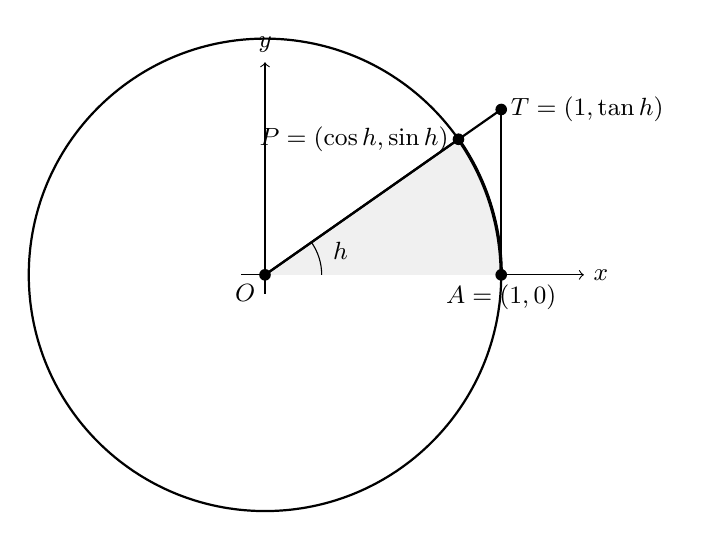
\begin{tikzpicture}[scale=3.0, every node/.style={font=\small}]
  % axes
  \draw[->] (-0.1,0) -- (1.35,0) node[right] {\(x\)};
  \draw[->] (0,-0.08) -- (0,0.9) node[above] {\(y\)};

  % unit circle arc
  \draw[thick] (0,0) circle (1);

  % fixed angle h = 35 degrees for picture
  \coordinate (O) at (0,0);
  \coordinate (A) at (1,0);
  \coordinate (P) at (0.819,0.574);
  \coordinate (T) at (1,0.700);

  % sector and triangles
  \fill[gray!12] (O) -- (A) arc[start angle=0,end angle=35,radius=1] -- cycle;
  \draw[thick] (O) -- (P);
  \draw[thick] (O) -- (T);
  \draw[thick] (A) -- (T);
  \draw[very thick] (A) arc[start angle=0,end angle=35,radius=1];

  % points
  \fill (O) circle (0.7pt) node[below left] {\(O\)};
  \fill (A) circle (0.7pt) node[below] {\(A=(1,0)\)};
  \fill (P) circle (0.7pt) node[left] {\(P=(\cos h,\sin h)\)};
  \fill (T) circle (0.7pt) node[right] {\(T=(1,\tan h)\)};

  % angle label
  \draw (0.24,0) arc[start angle=0,end angle=35,radius=0.24];
  \node at (0.32,0.10) {\(h\)};
\end{tikzpicture}
\caption{For \(0<h<\pi/2\), the small triangle lies inside the sector, which lies inside the larger triangle.}
\label{fig:sin-h-over-h-geometry}
\end{figure}

For \(0<h<\pi/2\), compare three areas in Figure \ref{fig:sin-h-over-h-geometry}:

\[
\text{area of } \triangle OAP
<
\text{area of sector } OAP
<
\text{area of } \triangle OAT.
\]

These areas are

\[
\frac12 \sin h,
\qquad
\frac12 h,
\qquad
\frac12 \tan h.
\]

So

\[
\frac12\sin h<\frac12h<\frac12\tan h.
\]

Multiplying by \(2\),

\[
\sin h<h<\tan h.
\]

Since \(\tan h=\dfrac{\sin h}{\cos h}\), we have

\[
\sin h<h<\frac{\sin h}{\cos h}.
\]

Divide by the positive number \(\sin h\):

\[
1<\frac{h}{\sin h}<\frac1{\cos h}.
\]

Taking reciprocals reverses the inequalities:

\[
\cos h<\frac{\sin h}{h}<1.
\]

As \(h\to0^+\),

\[
\cos h\to1.
\]

Therefore, by the Squeeze Theorem,

\[
\lim_{h\to0^+}\frac{\sin h}{h}=1.
\]

The function \(\dfrac{\sin h}{h}\) is even, because

\[
\frac{\sin(-h)}{-h}=\frac{\sin h}{h}.
\]

Thus the left-hand limit is the same as the right-hand limit.  Therefore

\[
\boxed{
\lim_{h\to0}\frac{\sin h}{h}=1.
}
\]

This limit is the small-angle fact behind the derivative of sine.  For very small \(h\), measured in radians,

\[
\sin h\approx h.
\]

On the unit circle, the vertical rise and the arc length are almost the same when the angle is tiny.

We will also need one companion limit:

\[
\lim_{h\to0}\frac{\cos h-1}{h}=0.
\]

Use the identity

\[
1-\cos h=2\sin^2\left(\frac h2\right).
\]

Then

\[
\frac{\cos h-1}{h}
=
-\frac{2\sin^2(h/2)}{h}
=
-\left(\frac{\sin(h/2)}{h/2}\right)\sin\left(\frac h2\right).
\]

As \(h\to0\),

\[
\frac{\sin(h/2)}{h/2}\to1
\]

and

\[
\sin\left(\frac h2\right)\to0.
\]

So

\[
\boxed{
\lim_{h\to0}\frac{\cos h-1}{h}=0.
}
\]

\subsection{The derivative of sine}
\label{subsec:derivative-sine}

Let

\[
f(x)=\sin x.
\]

We compute the derivative from the definition:

\[
f'(x)
=
\lim_{h\to0}\frac{\sin(x+h)-\sin x}{h}.
\]

Use the addition formula

\[
\sin(x+h)=\sin x\cos h+\cos x\sin h.
\]

Then

\[
\frac{\sin(x+h)-\sin x}{h}
=
\frac{\sin x\cos h+\cos x\sin h-\sin x}{h}.
\]

Group the terms:

\[
\frac{\sin(x+h)-\sin x}{h}
=
\sin x\left(\frac{\cos h-1}{h}\right)
+
\cos x\left(\frac{\sin h}{h}\right).
\]

Now take the limit:

\[
\frac{d}{dx}\sin x
=
\sin x\cdot0+\cos x\cdot1.
\]

Thus

\[
\boxed{
\frac{d}{dx}\sin x=\cos x.
}
\]

This formula has a simple geometric meaning.  At \(x=0\), the sine curve is rising with slope \(1\), and

\[
\cos0=1.
\]

At \(x=\pi/2\), the sine curve has a high point, so its slope is \(0\), and

\[
\cos\left(\frac{\pi}{2}\right)=0.
\]

At \(x=\pi\), the sine curve is falling with slope \(-1\), and

\[
\cos\pi=-1.
\]

\begin{figure}[h]
\centering
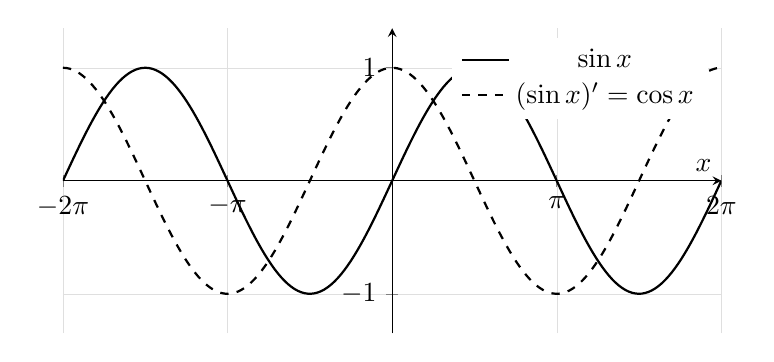
\begin{tikzpicture}
\begin{axis}[
    width=0.82\textwidth,
    height=0.45\textwidth,
    xmin=-6.283, xmax=6.283,
    ymin=-1.35, ymax=1.35,
    axis lines=middle,
    xlabel={\(x\)},
    ylabel={},
    xtick={-6.283,-3.142,0,3.142,6.283},
    xticklabels={\(-2\pi\),\(-\pi\),\(0\),\(\pi\),\(2\pi\)},
    ytick={-1,0,1},
    grid=both,
    grid style={line width=.1pt, draw=gray!25},
    legend style={draw=none, at={(0.98,0.97)}, anchor=north east}
]
\addplot[thick, domain=-6.283:6.283, samples=200] {sin(deg(x))};
\addlegendentry{\(\sin x\)}
\addplot[thick, dashed, domain=-6.283:6.283, samples=200] {cos(deg(x))};
\addlegendentry{\((\sin x)'=\cos x\)}
\end{axis}
\end{tikzpicture}
\caption{The derivative of the sine curve is the cosine curve.}
\label{fig:sine-derivative-cosine}
\end{figure}

\paragraph{Example.}
Differentiate

\[
y=x^2\sin x.
\]

Use the product rule:

\[
y'
=
2x\sin x+x^2\cos x.
\]

So

\[
\boxed{
\frac{d}{dx}\left(x^2\sin x\right)
=
2x\sin x+x^2\cos x.
}
\]

\paragraph{Example.}
Differentiate

\[
y=\sin(3x^2).
\]

The outside function is sine.  The inside function is

\[
u=3x^2.
\]

By the chain rule,

\[
y'=\cos(3x^2)\cdot 6x.
\]

Thus

\[
\boxed{
\frac{d}{dx}\sin(3x^2)=6x\cos(3x^2).
}
\]

\subsection{The derivative of cosine}
\label{subsec:derivative-cosine}

Cosine is a shifted sine:

\[
\cos x=\sin\left(\frac{\pi}{2}+x\right).
\]

Differentiate using the chain rule:

\[
\frac{d}{dx}\cos x
=
\frac{d}{dx}\sin\left(\frac{\pi}{2}+x\right).
\]

The derivative of sine is cosine, so

\[
\frac{d}{dx}\cos x
=
\cos\left(\frac{\pi}{2}+x\right)\cdot1.
\]

But

\[
\cos\left(\frac{\pi}{2}+x\right)=-\sin x.
\]

Therefore

\[
\boxed{
\frac{d}{dx}\cos x=-\sin x.
}
\]

The minus sign matters.  At \(x=0\), cosine has a high point, so the slope is \(0\).  At small positive \(x\), cosine is decreasing, so the slope is negative.  The formula

\[
(\cos x)'=-\sin x
\]

records exactly that.

\paragraph{Example.}
Differentiate

\[
y=\cos(5x-1).
\]

Let

\[
u=5x-1.
\]

Then

\[
y=\cos u.
\]

By the chain rule,

\[
y'=-\sin u\cdot u'.
\]

Since

\[
u'=5,
\]

we get

\[
\boxed{
y'=-5\sin(5x-1).
}
\]

\paragraph{Example.}
Differentiate

\[
f(t)=\sin t\cos t.
\]

Using the product rule,

\[
f'(t)
=
(\cos t)(\cos t)+(\sin t)(-\sin t).
\]

Thus

\[
f'(t)=\cos^2 t-\sin^2 t.
\]

Using the identity

\[
\cos(2t)=\cos^2t-\sin^2t,
\]

we can also write

\[
\boxed{
f'(t)=\cos(2t).
}
\]

This is a useful reminder: different-looking derivative answers can be the same after a trigonometric identity.

\subsection{Tangent, secant, cosecant, and cotangent}
\label{subsec:other-trig-derivatives}

The remaining trigonometric derivatives follow from sine and cosine together with the quotient and reciprocal rules.

Start with tangent:

\[
\tan x=\frac{\sin x}{\cos x}.
\]

By the quotient rule,

\[
\frac{d}{dx}\tan x
=
\frac{\cos x(\cos x)-\sin x(-\sin x)}{\cos^2x}.
\]

So

\[
\frac{d}{dx}\tan x
=
\frac{\cos^2x+\sin^2x}{\cos^2x}.
\]

Since

\[
\sin^2x+\cos^2x=1,
\]

we get

\[
\boxed{
\frac{d}{dx}\tan x=\sec^2x.
}
\]

Now use reciprocal forms.

Since

\[
\sec x=\frac1{\cos x},
\]

the reciprocal rule gives

\[
\frac{d}{dx}\sec x
=
-\frac{-\sin x}{\cos^2x}
=
\frac{\sin x}{\cos^2x}.
\]

Rewrite:

\[
\frac{\sin x}{\cos^2x}
=
\frac1{\cos x}\frac{\sin x}{\cos x}
=
\sec x\tan x.
\]

Thus

\[
\boxed{
\frac{d}{dx}\sec x=\sec x\tan x.
}
\]

Similarly,

\[
\csc x=\frac1{\sin x}.
\]

Therefore

\[
\frac{d}{dx}\csc x
=
-\frac{\cos x}{\sin^2x}
=
-\csc x\cot x.
\]

So

\[
\boxed{
\frac{d}{dx}\csc x=-\csc x\cot x.
}
\]

Finally,

\[
\cot x=\frac{\cos x}{\sin x}.
\]

Using the quotient rule,

\[
\frac{d}{dx}\cot x
=
\frac{\sin x(-\sin x)-\cos x(\cos x)}{\sin^2x}
=
-\frac{\sin^2x+\cos^2x}{\sin^2x}.
\]

Thus

\[
\boxed{
\frac{d}{dx}\cot x=-\csc^2x.
}
\]

We collect the six formulas:

\[
\boxed{
\begin{array}{c|c}
\text{function} & \text{derivative} \\ \hline
\sin x & \cos x \\[3pt]
\cos x & -\sin x \\[3pt]
\tan x & \sec^2x \\[3pt]
\sec x & \sec x\tan x \\[3pt]
\csc x & -\csc x\cot x \\[3pt]
\cot x & -\csc^2x
\end{array}
}
\]

The negative signs belong to the cofunctions:

\[
\cos x,\qquad \csc x,\qquad \cot x.
\]

That is a useful memory aid, but the formulas should also make sense from the graphs.

\paragraph{Example.}
Differentiate

\[
y=\frac{\cos x}{1+\sin x}.
\]

Use the quotient rule:

\[
y'
=
\frac{(1+\sin x)(-\sin x)-\cos x(\cos x)}{(1+\sin x)^2}.
\]

Expand the numerator:

\[
-\sin x-\sin^2x-\cos^2x.
\]

Since

\[
\sin^2x+\cos^2x=1,
\]

the numerator becomes

\[
-\sin x-1=-(1+\sin x).
\]

Therefore

\[
y'
=
-\frac{1+\sin x}{(1+\sin x)^2}
=
-\frac1{1+\sin x}.
\]

So

\[
\boxed{
\frac{d}{dx}\left(\frac{\cos x}{1+\sin x}\right)
=
-\frac1{1+\sin x}.
}
\]

This derivative exists wherever the original function exists, so we exclude points where

\[
1+\sin x=0.
\]

That happens when

\[
\sin x=-1,
\]

or

\[
x=\frac{3\pi}{2}+2\pi k,
\qquad k\in\mathbb Z.
\]

\subsection{Why radians are required}
\label{subsec:radians-required}

The formulas

\[
\frac{d}{dx}\sin x=\cos x
\qquad\text{and}\qquad
\frac{d}{dx}\cos x=-\sin x
\]

are true when \(x\) is measured in radians.

If \(x\) is measured in degrees, then the function

\[
S(x)=\sin(x^\circ)
\]

really means

\[
S(x)=\sin\left(\frac{\pi x}{180}\right).
\]

By the chain rule,

\[
S'(x)
=
\cos\left(\frac{\pi x}{180}\right)\cdot\frac{\pi}{180}.
\]

So

\[
\boxed{
\frac{d}{dx}\sin(x^\circ)
=
\frac{\pi}{180}\cos(x^\circ).
}
\]

The extra factor \(\pi/180\) appears because one degree is only \(\pi/180\) radians.

\begin{quote}
\textbf{Warning.}
The standard trigonometric derivative formulas assume radian measure.  Radians are not a convention added later.  They are the unit in which small angle and small arc length agree.
\end{quote}

\subsection{A preview of simple harmonic motion}
\label{subsec:simple-harmonic-motion-preview}

A spring gives a concrete reason why sine and cosine derivatives matter.

Suppose a mass hangs from a spring.  Pull it down \(4\) centimeters from its resting position and release it.  A simple model for its position is

\[
s(t)=4\cos(2t),
\]

where \(t\) is measured in seconds and \(s(t)\) is measured in centimeters from the rest position.  Positive \(s\) means downward.

The velocity is

\[
v(t)=s'(t).
\]

Using the chain rule,

\[
v(t)=4\cdot(-\sin(2t))\cdot2.
\]

So

\[
\boxed{
v(t)=-8\sin(2t).
}
\]

The acceleration is

\[
a(t)=v'(t).
\]

Differentiate again:

\[
a(t)=-8\cdot\cos(2t)\cdot2.
\]

Thus

\[
a(t)=-16\cos(2t).
\]

But

\[
s(t)=4\cos(2t),
\]

so

\[
a(t)=-4s(t).
\]

Therefore

\[
\boxed{
a(t)=-4s(t).
}
\]

The acceleration points opposite the displacement.  When the mass is below its rest position, the acceleration points upward.  When it is above its rest position, the acceleration points downward.  The spring pulls back toward equilibrium.

\begin{figure}[h]
\centering
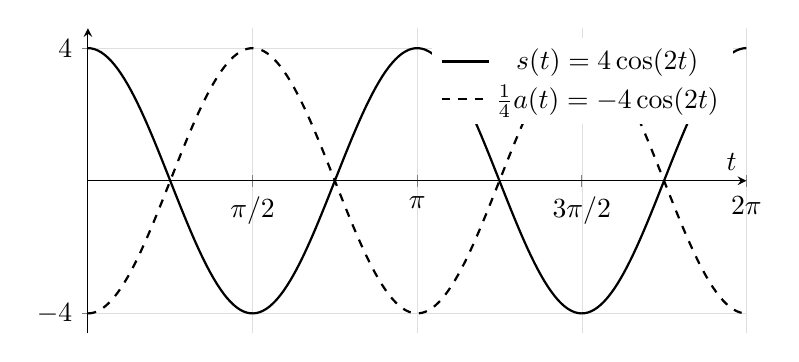
\begin{tikzpicture}
\begin{axis}[
    width=0.82\textwidth,
    height=0.45\textwidth,
    xmin=0, xmax=6.283,
    ymin=-4.6, ymax=4.6,
    axis lines=middle,
    xlabel={\(t\)},
    ylabel={},
    xtick={0,1.571,3.142,4.712,6.283},
    xticklabels={\(0\),\(\pi/2\),\(\pi\),\(3\pi/2\),\(2\pi\)},
    ytick={-4,0,4},
    grid=both,
    grid style={line width=.1pt, draw=gray!25},
    legend style={draw=none, at={(0.98,0.97)}, anchor=north east}
]
\addplot[thick, domain=0:6.283, samples=200] {4*cos(deg(2*x))};
\addlegendentry{\(s(t)=4\cos(2t)\)}
\addplot[thick, dashed, domain=0:6.283, samples=200] {-4*cos(deg(2*x))};
\addlegendentry{\(\frac14a(t)=-4\cos(2t)\)}
\end{axis}
\end{tikzpicture}
\caption{For simple harmonic motion, acceleration is proportional to displacement and points in the opposite direction.}
\label{fig:simple-harmonic-motion-preview}
\end{figure}

This is the first glimpse of a differential equation:

\[
s''(t)=-4s(t).
\]

It says the law of motion in terms of derivatives.  Later we will study such equations directly.  For now, the important point is that sine and cosine are built for repeated motion because their derivatives cycle back to sine and cosine.

Trigonometric functions describe quantities that repeat.  Another family describes quantities that grow or decay by multiplying: populations, radioactive substances, and continuously compounded money.  Their derivatives lead to the number \(e\).

\section{Derivatives of exponential and logarithmic functions}
\label{sec:derivatives-exponential-logarithmic}

Sine and cosine return to themselves after differentiation, with a shift and a sign.  Exponential functions are even more direct.  The right exponential function returns exactly to itself.

That one fact explains why exponentials appear whenever the rate of change depends on the current amount.

\subsection{Exponential growth as a rate law}
\label{subsec:exponential-growth-rate-law}

Imagine a small colony of bacteria.  If there are more bacteria, there are more bacteria able to divide.  So the growth rate should depend on the current population.

A simple model says

\[
P'(t)=kP(t),
\]

where

\[
P(t)
\]

is the population at time \(t\), and \(k\) is a constant.

If \(k>0\), the population grows.  If \(k<0\), the quantity decays.  The same equation appears in radioactive decay, continuous interest, and many first approximations to growth.

The equation

\[
P'(t)=kP(t)
\]

asks for a function whose derivative is a constant multiple of itself.

We already know one kind of candidate:

\[
P(t)=a^t.
\]

To see what its derivative looks like, use the definition:

\[
\frac{d}{dt}a^t
=
\lim_{h\to0}\frac{a^{t+h}-a^t}{h}.
\]

Using the exponent rule

\[
a^{t+h}=a^t a^h,
\]

we get

\[
\frac{a^{t+h}-a^t}{h}
=
\frac{a^t a^h-a^t}{h}
=
a^t\frac{a^h-1}{h}.
\]

Since \(a^t\) does not depend on \(h\),

\[
\frac{d}{dt}a^t
=
a^t\lim_{h\to0}\frac{a^h-1}{h}.
\]

The limit

\[
\lim_{h\to0}\frac{a^h-1}{h}
\]

is the slope of the graph \(y=a^x\) at \(x=0\).  Call that number \(\lambda(a)\):

\[
\lambda(a)=\lim_{h\to0}\frac{a^h-1}{h}.
\]

Then

\[
\boxed{
\frac{d}{dx}a^x=\lambda(a)a^x.
}
\]

Every exponential function has a derivative proportional to itself.  The proportionality constant depends on the base.

The natural question is:

\[
\text{Is there a base for which the proportionality constant is }1?
\]

Yes.  That base is \(e\).

\subsection{The special base \texorpdfstring{\(e\)}{e}}
\label{subsec:special-base-e}

The number \(e\) is the base for which

\[
\lim_{h\to0}\frac{e^h-1}{h}=1.
\]

Equivalently, the graph of \(y=e^x\) has slope \(1\) at \(x=0\).

Since

\[
e^0=1,
\]

the tangent line to \(y=e^x\) at \(x=0\) is

\[
y=1+x.
\]

\begin{figure}[h]
\centering
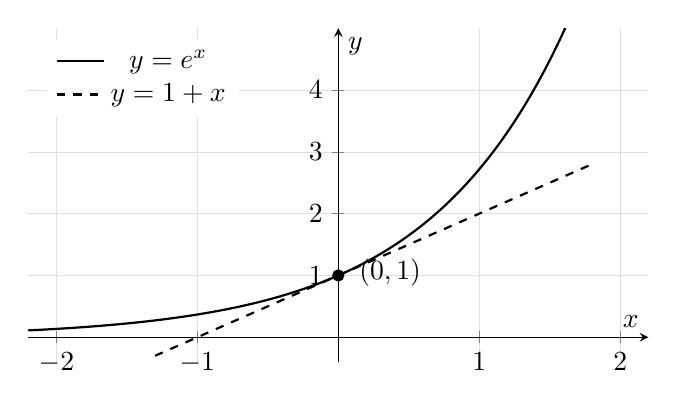
\begin{tikzpicture}
\begin{axis}[
    width=0.78\textwidth,
    height=0.48\textwidth,
    xmin=-2.2, xmax=2.2,
    ymin=-0.4, ymax=5.0,
    axis lines=middle,
    xlabel={\(x\)},
    ylabel={\(y\)},
    xtick={-2,-1,0,1,2},
    ytick={0,1,2,3,4},
    grid=both,
    grid style={line width=.1pt, draw=gray!25},
    legend style={draw=none, at={(0.03,0.97)}, anchor=north west}
]
\addplot[thick, domain=-2.2:2.2, samples=200] {exp(x)};
\addlegendentry{\(y=e^x\)}
\addplot[thick, dashed, domain=-1.3:1.8, samples=2] {1+x};
\addlegendentry{\(y=1+x\)}
\addplot[only marks, mark=*] coordinates {(0,1)};
\node[anchor=west] at (axis cs:0.08,1.05) {\((0,1)\)};
\end{axis}
\end{tikzpicture}
\caption{The base \(e\) is chosen so that \(e^x\) has slope \(1\) at \(x=0\).}
\label{fig:exponential-tangent-at-zero}
\end{figure}

This choice may look small, but it controls the whole function.  From the formula above,

\[
\frac{d}{dx}e^x
=
e^x\lim_{h\to0}\frac{e^h-1}{h}.
\]

The limit is \(1\), so

\[
\boxed{
\frac{d}{dx}e^x=e^x.
}
\]

The function \(e^x\) is its own derivative.

\subsection{The derivative of \texorpdfstring{\(e^{u(x)}\)}{e to u of x}}
\label{subsec:derivative-e-to-u}

The chain rule immediately extends this formula.

If

\[
y=e^{u(x)},
\]

then the outside derivative is

\[
\frac{d}{du}e^u=e^u,
\]

and the inside derivative is

\[
u'(x).
\]

Thus

\[
\boxed{
\frac{d}{dx}e^{u(x)}=e^{u(x)}u'(x).
}
\]

\paragraph{Example.}
Differentiate

\[
y=e^{-x^2}.
\]

Let

\[
u=-x^2.
\]

Then

\[
u'=-2x.
\]

Therefore

\[
\boxed{
y'=-2xe^{-x^2}.
}
\]

This derivative is positive when \(x<0\), zero when \(x=0\), and negative when \(x>0\).  So \(e^{-x^2}\) rises to a peak at \(x=0\) and falls afterward.

\paragraph{Example.}
Differentiate

\[
y=x^2e^{3x}.
\]

Use the product rule:

\[
y'
=
2xe^{3x}+x^2\frac{d}{dx}e^{3x}.
\]

By the chain rule,

\[
\frac{d}{dx}e^{3x}=3e^{3x}.
\]

So

\[
y'=2xe^{3x}+3x^2e^{3x}.
\]

Factor:

\[
\boxed{
y'=xe^{3x}(2+3x).
}
\]

\subsection{The derivative of \texorpdfstring{\(a^x\)}{a to x}}
\label{subsec:derivative-a-to-x}

Every positive base \(a\) can be written using \(e\).  Since \(\ln a\) is the exponent that produces \(a\),

\[
a=e^{\ln a}.
\]

Therefore

\[
a^x=\left(e^{\ln a}\right)^x=e^{x\ln a}.
\]

Differentiate:

\[
\frac{d}{dx}a^x
=
\frac{d}{dx}e^{x\ln a}.
\]

Here \(\ln a\) is a constant, so the chain rule gives

\[
\frac{d}{dx}a^x
=
e^{x\ln a}\cdot\ln a.
\]

Since

\[
e^{x\ln a}=a^x,
\]

we get

\[
\boxed{
\frac{d}{dx}a^x=(\ln a)a^x,
\qquad a>0.
}
\]

If \(a>1\), then

\[
\ln a>0,
\]

so \(a^x\) is increasing.

If \(0<a<1\), then

\[
\ln a<0,
\]

so \(a^x\) is decreasing.

The formula includes both growth and decay.

\paragraph{Example.}
Differentiate

\[
y=10^x.
\]

Using the formula,

\[
\boxed{
y'=(\ln 10)10^x.
}
\]

The graph of \(10^x\) is steeper than \(e^x\) at corresponding heights because

\[
\ln 10>1.
\]

\paragraph{Example.}
Differentiate

\[
y=2^{x^2+1}.
\]

Let

\[
u=x^2+1.
\]

Then

\[
y=2^u.
\]

The derivative of \(2^u\) with respect to \(u\) is

\[
(\ln2)2^u.
\]

So the chain rule gives

\[
y'
=
(\ln2)2^{x^2+1}\cdot 2x.
\]

Thus

\[
\boxed{
y'=2x(\ln2)2^{x^2+1}.
}
\]

\subsection{The derivative of \texorpdfstring{\(\ln x\)}{ln x}}
\label{subsec:derivative-ln-x}

The natural logarithm is the inverse of the natural exponential function.

That means

\[
y=\ln x
\]

is equivalent to

\[
x=e^y.
\]

We can find the derivative of \(\ln x\) using implicit differentiation.

Start with

\[
x=e^y.
\]

Differentiate both sides with respect to \(x\):

\[
1=e^y\frac{dy}{dx}.
\]

Since

\[
e^y=x,
\]

we get

\[
1=x\frac{dy}{dx}.
\]

Therefore

\[
\frac{dy}{dx}=\frac1x.
\]

Thus

\[
\boxed{
\frac{d}{dx}\ln x=\frac1x,
\qquad x>0.
}
\]

The condition \(x>0\) is part of the formula.  In real-valued calculus, \(\ln x\) is defined only for positive \(x\).

\paragraph{Example.}
Differentiate

\[
y=\ln(3x^2+1).
\]

Let

\[
u=3x^2+1.
\]

Then

\[
y=\ln u.
\]

By the chain rule,

\[
y'=\frac1u u'.
\]

Since

\[
u'=6x,
\]

we get

\[
\boxed{
y'=\frac{6x}{3x^2+1}.
}
\]

More generally,

\[
\boxed{
\frac{d}{dx}\ln(u(x))=\frac{u'(x)}{u(x)}
}
\]

where \(u(x)>0\).

\paragraph{Example.}
Differentiate

\[
y=\ln(\sin x).
\]

The function is defined where

\[
\sin x>0.
\]

On such intervals,

\[
y'=\frac{\cos x}{\sin x}.
\]

So

\[
\boxed{
\frac{d}{dx}\ln(\sin x)=\cot x
}
\]

where \(\sin x>0\).

\paragraph{A useful extension.}
On intervals where \(u(x)\neq0\), the function \(\ln|u(x)|\) is defined, and

\[
\boxed{
\frac{d}{dx}\ln|u(x)|=\frac{u'(x)}{u(x)}.
}
\]

For example,

\[
\frac{d}{dx}\ln|x^2-1|
=
\frac{2x}{x^2-1},
\qquad x\neq\pm1.
\]

The absolute value lets us use logarithms on intervals where \(u(x)\) is negative, but it still cannot cross through \(u(x)=0\).  The logarithm has no finite value there.

\subsection{Logarithms with other bases}
\label{subsec:derivative-log-base-a}

For \(a>0\) and \(a\neq1\), the logarithm base \(a\) satisfies

\[
\log_a x=\frac{\ln x}{\ln a}.
\]

Since \(\ln a\) is a constant,

\[
\frac{d}{dx}\log_a x
=
\frac1{\ln a}\frac{d}{dx}\ln x.
\]

Therefore

\[
\boxed{
\frac{d}{dx}\log_a x=\frac1{x\ln a},
\qquad x>0,\ a>0,\ a\neq1.
}
\]

Natural logarithms dominate calculus because their derivative is simplest:

\[
(\ln x)'=\frac1x.
\]

Other logarithms carry the extra constant

\[
\frac1{\ln a}.
\]

\subsection{Logarithmic differentiation}
\label{subsec:logarithmic-differentiation}

Some functions are awkward for ordinary differentiation rules.  They involve many factors, powers, or variables in both the base and the exponent.

For example,

\[
y=x^x
\]

has \(x\) in the base and in the exponent.  It is not a power function like \(x^5\), and it is not an exponential function like \(5^x\).

Take logarithms:

\[
\ln y=\ln(x^x).
\]

Using logarithm rules,

\[
\ln y=x\ln x.
\]

Now differentiate both sides with respect to \(x\).  Since \(y\) depends on \(x\), the left side requires the chain rule:

\[
\frac{d}{dx}\ln y=\frac1y\frac{dy}{dx}.
\]

The right side uses the product rule:

\[
\frac{d}{dx}(x\ln x)=\ln x+x\cdot\frac1x=\ln x+1.
\]

So

\[
\frac1y\frac{dy}{dx}=\ln x+1.
\]

Multiply by \(y\):

\[
\frac{dy}{dx}=y(\ln x+1).
\]

Since

\[
y=x^x,
\]

we get

\[
\boxed{
\frac{d}{dx}x^x=x^x(\ln x+1),
\qquad x>0.
}
\]

This method is called \emph{logarithmic differentiation}.

\begin{quote}
\textbf{Logarithmic differentiation.}
When a positive function \(y=f(x)\) is a product, quotient, power, or variable-base expression, it can help to take natural logarithms first:

\[
\ln y=\ln(f(x)).
\]

Then differentiate implicitly and solve for \(y'\).
\end{quote}

\paragraph{Example.}
Differentiate

\[
y=\frac{(x^2+1)^5\sqrt{x-1}}{(3x+2)^4},
\qquad x>1.
\]

Taking natural logarithms gives

\[
\ln y
=
\ln\left(\frac{(x^2+1)^5\sqrt{x-1}}{(3x+2)^4}\right).
\]

Use logarithm rules:

\[
\ln y
=
5\ln(x^2+1)+\frac12\ln(x-1)-4\ln(3x+2).
\]

Differentiate both sides:

\[
\frac{y'}{y}
=
5\cdot\frac{2x}{x^2+1}
+
\frac12\cdot\frac1{x-1}
-
4\cdot\frac3{3x+2}.
\]

So

\[
\frac{y'}{y}
=
\frac{10x}{x^2+1}
+
\frac1{2(x-1)}
-
\frac{12}{3x+2}.
\]

Multiply by \(y\):

\[
y'
=
y\left(
\frac{10x}{x^2+1}
+
\frac1{2(x-1)}
-
\frac{12}{3x+2}
\right).
\]

Substitute the original expression for \(y\):

\[
\boxed{
y'
=
\frac{(x^2+1)^5\sqrt{x-1}}{(3x+2)^4}
\left(
\frac{10x}{x^2+1}
+
\frac1{2(x-1)}
-
\frac{12}{3x+2}
\right).
}
\]

Without logarithmic differentiation, this derivative would require several rounds of product, quotient, and chain rules.  The logarithm turns products into sums and powers into coefficients.

\paragraph{Example.}
Differentiate

\[
y=(\sin x)^x,
\]

on an interval where

\[
\sin x>0.
\]

Take logarithms:

\[
\ln y=x\ln(\sin x).
\]

Differentiate:

\[
\frac{y'}{y}
=
\ln(\sin x)+x\frac{\cos x}{\sin x}.
\]

Thus

\[
\frac{y'}{y}
=
\ln(\sin x)+x\cot x.
\]

Multiply by \(y\):

\[
\boxed{
y'
=
(\sin x)^x\left(\ln(\sin x)+x\cot x\right).
}
\]

The condition \(\sin x>0\) matters.  The expression \((\sin x)^x\) is not a real-valued elementary function for all real \(x\), and \(\ln(\sin x)\) only makes sense where \(\sin x\) is positive.

\subsection{The derivative table so far}
\label{subsec:derivative-table-so-far}

We now have the main elementary derivative formulas:

\[
\boxed{
\begin{array}{c|c}
\text{function} & \text{derivative} \\ \hline
x^n & nx^{n-1} \\[3pt]
\sin x & \cos x \\[3pt]
\cos x & -\sin x \\[3pt]
\tan x & \sec^2x \\[3pt]
e^x & e^x \\[3pt]
a^x & (\ln a)a^x \\[3pt]
\ln x & \dfrac1x \\[8pt]
\log_a x & \dfrac1{x\ln a}
\end{array}
}
\]

Together with the sum, product, quotient, and chain rules, these formulas let us differentiate a wide range of functions.

But one idea has appeared twice without being named fully.  We found \(\ln x\) by reversing \(e^x\).  Earlier, trigonometry gave us sine and cosine; reversing those functions will give \(\arcsin x\), \(\arccos x\), and \(\arctan x\).  The next question is general: when a function has an inverse, how is the derivative of the inverse related to the original derivative?
\section{Derivatives of trigonometric functions}\Core
\label{sec:deriv-trig}

The chain rule taught us how change passes through a composition, and implicit
differentiation let us find slopes on curves that were not solved for one variable.
But many motions are not built from powers and algebraic operations. They repeat.

Imagine a point moving counterclockwise around the unit circle at one radian per
second. Its height is

\[
\sin t,
\]

and its horizontal coordinate is

\[
\cos t.
\]

At the rightmost point, the height is rising as fast as possible. At the top, the
height stops changing for an instant. At the leftmost point, the height is falling as
fast as possible. The horizontal coordinate records exactly this pattern. This suggests

\[
\frac{d}{dt}\sin t=\cos t.
\]

To prove that formula, we need one geometric fact about very small angles.

\subsection{Radians and the limit \texorpdfstring{$\sin h/h\to 1$}{sin h / h -> 1}}
\label{subsec:radians-sinhh}

Earlier, radians were defined by arc length:

\[
\text{angle in radians}
=
\frac{\text{arc length}}{\text{radius}}.
\]

On the unit circle, the radius is \(1\). Therefore an angle of \(h\) radians cuts off
an arc of length \(h\). This direct agreement between angle and length is what makes
radians the natural unit for differentiation.

For \(0<h<\pi/2\), let

\[
A=(1,0),
\qquad
P=(\cos h,\sin h),
\]

and let the ray from the origin through \(P\) meet the tangent line \(x=1\) at

\[
T=(1,\tan h).
\]

\begin{figure}[h]
\centering
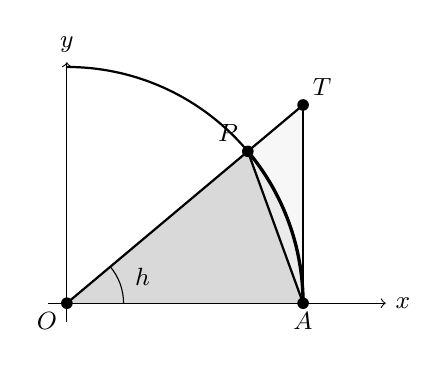
\begin{tikzpicture}[scale=3.0, every node/.style={font=\small}]
  \def\ang{40}

  \coordinate (O) at (0,0);
  \coordinate (A) at (1,0);
  \coordinate (P) at ({cos(\ang)},{sin(\ang)});
  \coordinate (T) at (1,{tan(\ang)});

  % The three nested regions: outer triangle, sector, inner triangle.
  \fill[gray!6] (O) -- (A) -- (T) -- cycle;
  \fill[gray!16] (O) -- (A)
      arc[start angle=0,end angle=\ang,radius=1] -- cycle;
  \fill[gray!30] (O) -- (A) -- (P) -- cycle;

  \draw[->] (-0.08,0) -- (1.35,0) node[right] {\(x\)};
  \draw[->] (0,-0.08) -- (0,1.02) node[above] {\(y\)};

  \draw[thick] (A) arc[start angle=0,end angle=90,radius=1];
  \draw[thick] (O) -- (T);
  \draw[thick] (A) -- (T);
  \draw[thick] (A) -- (P);
  \draw[very thick] (A)
      arc[start angle=0,end angle=\ang,radius=1];

  \fill (O) circle (0.7pt) node[below left] {\(O\)};
  \fill (A) circle (0.7pt) node[below] {\(A\)};
  \fill (P) circle (0.7pt) node[above left] {\(P\)};
  \fill (T) circle (0.7pt) node[above right] {\(T\)};

  \draw (0.24,0) arc[start angle=0,end angle=\ang,radius=0.24];
  \node at (0.32,0.11) {\(h\)};
\end{tikzpicture}
\caption{For \(0<h<\pi/2\), the inner triangle lies inside the circular sector, and the sector lies inside the outer triangle.}
\label{fig:sin-h-over-h-geometry}
\end{figure}

The three regions in Figure \ref{fig:sin-h-over-h-geometry} satisfy

\[
\operatorname{area}(\triangle OAP)
<
\operatorname{area}(\text{sector }OAP)
<
\operatorname{area}(\triangle OAT).
\]

Their areas are easy to compute.

The inner triangle has base \(OA=1\) and height \(\sin h\), so

\[
\operatorname{area}(\triangle OAP)=\frac12\sin h.
\]

The unit-circle sector has area

\[
\frac12h.
\]

This formula uses radians: the sector is \(h/(2\pi)\) of the full unit disk, whose
area is \(\pi\).

The outer triangle has base \(OA=1\) and height \(\tan h\), so

\[
\operatorname{area}(\triangle OAT)=\frac12\tan h.
\]

Therefore

\[
\frac12\sin h
<
\frac12h
<
\frac12\tan h,
\]

and hence

\[
\sin h<h<\tan h.
\]

Because \(0<h<\pi/2\), both \(\sin h\) and \(\cos h\) are positive. Using

\[
\tan h=\frac{\sin h}{\cos h},
\]

we obtain

\[
1<\frac{h}{\sin h}<\frac1{\cos h}.
\]

Taking reciprocals reverses the inequalities:

\[
\cos h<\frac{\sin h}{h}<1.
\]

As \(h\to0^+\), continuity of cosine gives

\[
\cos h\to1.
\]

The Squeeze Theorem therefore gives

\[
\lim_{h\to0^+}\frac{\sin h}{h}=1.
\]

The function \(\sin h/h\) is even, because

\[
\frac{\sin(-h)}{-h}=\frac{\sin h}{h}.
\]

Thus the left-hand limit is the same as the right-hand limit, and

\[
\boxed{
\lim_{h\to0}\frac{\sin h}{h}=1.
}
\]

This is the small-angle limit. It says that, for a tiny angle measured in radians,

\[
\sin h\approx h.
\]

More precisely,

\[
\frac{\sin h-h}{h}\to0.
\]

So the error in replacing \(\sin h\) by \(h\) is small compared with \(h\) itself.

We also need a companion limit. The half-angle identity gives

\[
1-\cos h=2\sin^2\left(\frac h2\right).
\]

Therefore

\[
\frac{\cos h-1}{h}
=
-\frac{2\sin^2(h/2)}{h}
=
-\left(\frac{\sin(h/2)}{h/2}\right)
 \sin\left(\frac h2\right).
\]

As \(h\to0\), the first factor approaches \(1\), and the second approaches \(0\).
Hence

\[
\boxed{
\lim_{h\to0}\frac{\cos h-1}{h}=0.
}
\]

\paragraph{Why degrees change the answer.}
Suppose the number \(h\) is interpreted as a degree measure. Then

\[
\sin(h^\circ)
=
\sin\left(\frac{\pi h}{180}\right).
\]

Consequently,

\[
\frac{\sin(h^\circ)}{h}
=
\frac{\pi}{180}
\frac{\sin(\pi h/180)}{\pi h/180}.
\]

Letting \(h\to0\) gives

\[
\lim_{h\to0}\frac{\sin(h^\circ)}{h}
=
\frac{\pi}{180},
\]

not \(1\). The clean trigonometric derivative formulas require radians.


\subsection{Derivative of sine}
\label{subsec:deriv-sine}

The small-angle limit first gives the slope of sine at the origin:

\[
\left.\frac{d}{dx}\sin x\right|_{x=0}
=
\lim_{h\to0}\frac{\sin h-\sin0}{h}
=
\lim_{h\to0}\frac{\sin h}{h}
=
1.
\]

That agrees with the unit-circle picture: at the rightmost point, the vertical
coordinate is rising at unit rate. The general slope follows from the addition formula.

\begin{quote}
\textbf{Derivative of sine.}
When \(x\) is measured in radians,

\[
\boxed{
\frac{d}{dx}\sin x=\cos x.
}
\]
\end{quote}

\paragraph{Proof.}
By the definition of derivative,

\[
\frac{d}{dx}\sin x
=
\lim_{h\to0}
\frac{\sin(x+h)-\sin x}{h}.
\]

Use

\[
\sin(x+h)=\sin x\cos h+\cos x\sin h.
\]

Then

\begin{align*}
\frac{\sin(x+h)-\sin x}{h}
&=
\frac{\sin x\cos h+\cos x\sin h-\sin x}{h}
\\
&=
\sin x\left(\frac{\cos h-1}{h}\right)
+
\cos x\left(\frac{\sin h}{h}\right).
\end{align*}

Taking the limit gives

\[
\frac{d}{dx}\sin x
=
\sin x\cdot0+\cos x\cdot1
=
\cos x.
\]

The formula can also be read as a local linear approximation:

\[
\boxed{
\sin(x+h)
\approx
\sin x+\cos x\,h
}
\]

for small \(h\).

\begin{figure}[h]
\centering
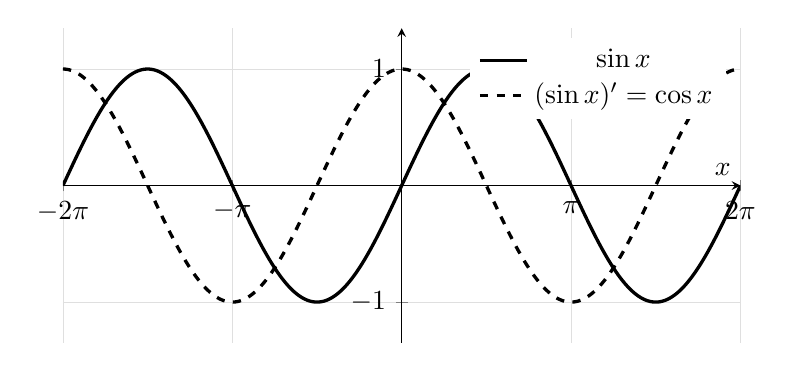
\begin{tikzpicture}
\begin{axis}[
    width=0.84\textwidth,
    height=0.46\textwidth,
    xmin=-6.283, xmax=6.283,
    ymin=-1.35, ymax=1.35,
    axis lines=middle,
    xlabel={\(x\)},
    ylabel={},
    xtick={-6.283,-3.142,0,3.142,6.283},
    xticklabels={\(-2\pi\),\(-\pi\),\(0\),\(\pi\),\(2\pi\)},
    ytick={-1,0,1},
    grid=both,
    grid style={line width=.1pt, draw=gray!25},
    legend style={
        draw=none,
        at={(0.98,0.97)},
        anchor=north east
    }
]
\addplot[
    very thick,
    domain=-6.283:6.283,
    samples=300
]
{sin(deg(x))};
\addlegendentry{\(\sin x\)}

\addplot[
    very thick,
    dashed,
    domain=-6.283:6.283,
    samples=300
]
{cos(deg(x))};
\addlegendentry{\((\sin x)'=\cos x\)}
\end{axis}
\end{tikzpicture}
\caption{The cosine graph records the slope of the sine graph. Its zeros occur where sine has horizontal tangents.}
\label{fig:sine-derivative-cosine}
\end{figure}

The graph matches the formula. At \(x=0\), sine rises with slope \(1\), and

\[
\cos0=1.
\]

At \(x=\pi/2\), sine has a high point, and

\[
\cos\left(\frac{\pi}{2}\right)=0.
\]

At \(x=\pi\), sine falls with slope \(-1\), and

\[
\cos\pi=-1.
\]

\paragraph{Example: product and trigonometric change.}
Differentiate

\[
y=x^2\sin x.
\]

Both factors change, so we use the product rule:

\[
y'
=
2x\sin x+x^2\cos x.
\]

Thus

\[
\boxed{
\frac{d}{dx}\left(x^2\sin x\right)
=
2x\sin x+x^2\cos x.
}
\]

\paragraph{Example: sine of an inside function.}
Differentiate

\[
y=\sin(3x^2).
\]

The outside function is sine, and the inside function is

\[
u=3x^2.
\]

The chain rule gives

\[
y'
=
\cos(3x^2)\cdot6x.
\]

Therefore

\[
\boxed{
y'=6x\cos(3x^2).
}
\]

If an angle is entered in degrees instead, the chain rule produces a conversion
factor. For

\[
S(x)=\sin\left(\frac{\pi x}{180}\right),
\]

we have

\[
S'(x)
=
\frac{\pi}{180}
\cos\left(\frac{\pi x}{180}\right).
\]

This is the derivative of the degree-based sine function, not \(\cos x\).

\subsection{Derivative of cosine}
\label{subsec:deriv-cosine}

At the origin, cosine has a horizontal tangent. The companion limit confirms this:

\[
\left.\frac{d}{dx}\cos x\right|_{x=0}
=
\lim_{h\to0}\frac{\cos h-1}{h}
=
0.
\]

As \(x\) increases from \(0\), cosine decreases. So its derivative should be negative.
The addition formula gives the exact pattern.

\begin{quote}
\textbf{Derivative of cosine.}
When \(x\) is measured in radians,

\[
\boxed{
\frac{d}{dx}\cos x=-\sin x.
}
\]
\end{quote}

\paragraph{Proof.}
Start from the difference quotient:

\[
\frac{d}{dx}\cos x
=
\lim_{h\to0}
\frac{\cos(x+h)-\cos x}{h}.
\]

Use

\[
\cos(x+h)=\cos x\cos h-\sin x\sin h.
\]

Then

\begin{align*}
\frac{\cos(x+h)-\cos x}{h}
&=
\frac{\cos x\cos h-\sin x\sin h-\cos x}{h}
\\
&=
\cos x\left(\frac{\cos h-1}{h}\right)
-
\sin x\left(\frac{\sin h}{h}\right).
\end{align*}

Taking the limit gives

\[
\frac{d}{dx}\cos x
=
\cos x\cdot0-\sin x\cdot1
=
-\sin x.
\]

Thus the local linear approximation is

\[
\boxed{
\cos(x+h)
\approx
\cos x-\sin x\,h.
}
\]

There is also a phase-shift explanation. Since

\[
\cos x=\sin\left(x+\frac{\pi}{2}\right),
\]

the chain rule gives

\[
\frac{d}{dx}\cos x
=
\cos\left(x+\frac{\pi}{2}\right)
=
-\sin x.
\]

\paragraph{Example: cosine of a linear function.}
Differentiate

\[
y=\cos(5x-1).
\]

By the chain rule,

\[
y'
=
-\sin(5x-1)\cdot5.
\]

Therefore

\[
\boxed{
y'=-5\sin(5x-1).
}
\]

\paragraph{Example: product of sine and cosine.}
Let

\[
f(t)=\sin t\cos t.
\]

The product rule gives

\begin{align*}
f'(t)
&=
(\cos t)(\cos t)+(\sin t)(-\sin t)
\\
&=
\cos^2t-\sin^2t.
\end{align*}

Using the double-angle identity,

\[
\boxed{
f'(t)=\cos(2t).
}
\]

Different-looking derivative formulas can represent the same function. Trigonometric
identities remain part of the algebra.

\subsection{Tangent, secant, cosecant, and cotangent}
\label{subsec:deriv-other-trig}

The other four trigonometric derivatives now follow from the quotient and reciprocal
rules. No new limit is needed.

Start with

\[
\tan x=\frac{\sin x}{\cos x}.
\]

Where \(\cos x\neq0\), the quotient rule gives

\begin{align*}
\frac{d}{dx}\tan x
&=
\frac{\cos x(\cos x)-\sin x(-\sin x)}{\cos^2x}
\\
&=
\frac{\cos^2x+\sin^2x}{\cos^2x}
\\
&=
\frac1{\cos^2x}.
\end{align*}

Therefore

\[
\boxed{
\frac{d}{dx}\tan x=\sec^2x.
}
\]

Since

\[
\sec x=\frac1{\cos x},
\]

the reciprocal rule gives

\begin{align*}
\frac{d}{dx}\sec x
&=
-\frac{-\sin x}{\cos^2x}
\\
&=
\frac1{\cos x}\frac{\sin x}{\cos x}.
\end{align*}

Hence

\[
\boxed{
\frac{d}{dx}\sec x=\sec x\tan x.
}
\]

Similarly,

\[
\csc x=\frac1{\sin x},
\]

so

\[
\boxed{
\frac{d}{dx}\csc x=-\csc x\cot x.
}
\]

Finally,

\[
\cot x=\frac{\cos x}{\sin x}.
\]

Where \(\sin x\neq0\), the quotient rule gives

\begin{align*}
\frac{d}{dx}\cot x
&=
\frac{\sin x(-\sin x)-\cos x(\cos x)}{\sin^2x}
\\
&=
-\frac{\sin^2x+\cos^2x}{\sin^2x}
\\
&=
-\csc^2x.
\end{align*}

Thus

\[
\boxed{
\frac{d}{dx}\cot x=-\csc^2x.
}
\]

The six trigonometric derivatives are collected below.

\begin{center}
\renewcommand{\arraystretch}{1.35}
\begin{tabular}{c|c|c}
\textbf{function}
&
\textbf{derivative}
&
\textbf{where the function is defined}
\\ \hline
\(\sin x\)
&
\(\cos x\)
&
all real \(x\)
\\
\(\cos x\)
&
\(-\sin x\)
&
all real \(x\)
\\
\(\tan x\)
&
\(\sec^2x\)
&
\(\cos x\neq0\)
\\
\(\sec x\)
&
\(\sec x\tan x\)
&
\(\cos x\neq0\)
\\
\(\csc x\)
&
\(-\csc x\cot x\)
&
\(\sin x\neq0\)
\\
\(\cot x\)
&
\(-\csc^2x\)
&
\(\sin x\neq0\)
\end{tabular}
\end{center}

A derivative formula does not repair a missing input. For example, tangent and
secant are still undefined at

\[
x=\frac{\pi}{2}+k\pi,
\qquad
k\in\mathbb Z.
\]

Cosecant and cotangent are undefined at

\[
x=k\pi,
\qquad
k\in\mathbb Z.
\]

When a trigonometric function contains an inside function \(u=u(x)\), the chain
rule adds the factor \(u'(x)\). For example,

\[
\frac{d}{dx}\tan(u(x))
=
\sec^2(u(x))u'(x),
\]

and

\[
\frac{d}{dx}\sec(u(x))
=
\sec(u(x))\tan(u(x))u'(x).
\]

\paragraph{Example: secant with an inside function.}
Differentiate

\[
y=\sec(x^2).
\]

The outside derivative is \(\sec u\tan u\), and the inside derivative is \(2x\).
Hence

\[
\boxed{
y'=2x\sec(x^2)\tan(x^2).
}
\]

This formula is valid wherever

\[
\cos(x^2)\neq0.
\]

\paragraph{Example: simplification after differentiation.}
Differentiate

\[
y=\frac{\cos x}{1+\sin x}.
\]

The quotient rule gives

\[
y'
=
\frac{(1+\sin x)(-\sin x)-\cos^2x}{(1+\sin x)^2}.
\]

The numerator is

\[
-\sin x-\sin^2x-\cos^2x
=
-(1+\sin x).
\]

Therefore

\[
\boxed{
y'=-\frac1{1+\sin x}.
}
\]

The original function is undefined when \(1+\sin x=0\), so the derivative formula
has the same restriction.

\subsection{Simple harmonic motion preview}
\label{subsec:shm-preview}

A spring gives a concrete reason why sine and cosine return under differentiation.

Suppose a mass hangs from a vertical spring. Pull it \(4\) centimeters below its rest
position and release it. In an idealized model, its displacement is

\[
s(t)=4\cos(2t),
\]

where \(t\) is measured in seconds and positive displacement points downward. The
number \(2\) is the angular frequency, measured in radians per second.

The velocity is

\[
v(t)=s'(t).
\]

Using the chain rule,

\[
\boxed{
v(t)=-8\sin(2t)
}
\]

centimeters per second.

Differentiate once more to find acceleration:

\[
a(t)=v'(t)=-16\cos(2t).
\]

Since

\[
s(t)=4\cos(2t),
\]

we have

\[
\boxed{
a(t)=-4s(t).
}
\]

The acceleration is proportional to the displacement and points in the opposite
direction.

At \(t=0\), the mass is \(4\) centimeters below equilibrium. Its velocity is \(0\),
but its acceleration is negative, so it begins moving upward.

At \(t=\pi/4\), the mass passes through equilibrium:

\[
s\left(\frac{\pi}{4}\right)=0,
\qquad
v\left(\frac{\pi}{4}\right)=-8.
\]

Its speed is largest there.

At \(t=\pi/2\), the mass is \(4\) centimeters above equilibrium. It stops for an
instant, and the acceleration points downward.

\begin{figure}[h]
\centering
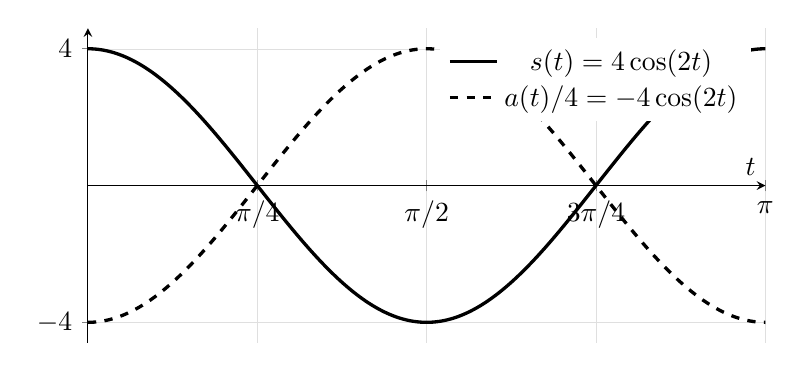
\begin{tikzpicture}
\begin{axis}[
    width=0.84\textwidth,
    height=0.46\textwidth,
    xmin=0, xmax=3.142,
    ymin=-4.6, ymax=4.6,
    axis lines=middle,
    xlabel={\(t\)},
    ylabel={},
    xtick={0,0.7854,1.5708,2.3562,3.1416},
    xticklabels={
        \(0\),
        \(\pi/4\),
        \(\pi/2\),
        \(3\pi/4\),
        \(\pi\)
    },
    ytick={-4,0,4},
    grid=both,
    grid style={line width=.1pt, draw=gray!25},
    legend style={
        draw=none,
        at={(0.98,0.97)},
        anchor=north east
    }
]
\addplot[
    very thick,
    domain=0:3.1416,
    samples=250
]
{4*cos(deg(2*x))};
\addlegendentry{\(s(t)=4\cos(2t)\)}

\addplot[
    very thick,
    dashed,
    domain=0:3.1416,
    samples=250
]
{-4*cos(deg(2*x))};
\addlegendentry{\(a(t)/4=-4\cos(2t)\)}
\end{axis}
\end{tikzpicture}
\caption{The displacement and the scaled acceleration have opposite signs. The spring always accelerates the mass back toward equilibrium.}
\label{fig:shm-displacement-acceleration}
\end{figure}

The same pattern holds for the general oscillation

\[
s(t)=A\cos(\omega t+\phi),
\qquad
\omega>0.
\]

Here \(|A|\) is the amplitude, \(\omega\) is the angular frequency, and \(\phi\)
shifts the timing of the motion. Differentiating twice gives

\[
s'(t)=-A\omega\sin(\omega t+\phi),
\]

and

\[
s''(t)=-A\omega^2\cos(\omega t+\phi).
\]

Therefore

\[
\boxed{
s''(t)=-\omega^2s(t).
}
\]

The period is

\[
\boxed{
T=\frac{2\pi}{\omega}.
}
\]

This is our first glimpse of a second-order differential equation. Later we will
reverse the question: if a law gives

\[
s''=-\omega^2s,
\]

why do sine and cosine appear in the solution?

Sine and cosine return to each other under differentiation. Growth and decay ask
for an even tighter pattern: a function that returns exactly to itself after one
derivative. That search leads to the exponential function.
\section{Inverse functions and inverse trigonometric functions}
\label{sec:inverse-functions-inverse-trig}

The last section found the derivative of \(\ln x\) by reversing the exponential function:

\[
y=\ln x
\qquad\Longleftrightarrow\qquad
x=e^y.
\]

That was not a special trick.  It was the first example of a general idea.

If a function can be reversed, then its derivative tells us the derivative of the reverse function.  The two slopes are reciprocals, but at corresponding points.

\subsection{The derivative of an inverse function}
\label{subsec:derivative-inverse-function}

Start with a simple increasing function:

\[
f(x)=x^3+x.
\]

Since

\[
f'(x)=3x^2+1>0
\]

for every \(x\), the function is always increasing.  So it passes the horizontal line test and has an inverse function.

Let

\[
g=f^{-1}.
\]

That means

\[
g(f(x))=x
\]

and

\[
f(g(y))=y.
\]

For example,

\[
f(1)=1^3+1=2,
\]

so

\[
g(2)=1.
\]

Now ask for the slope of the inverse function at \(y=2\).  Since the original function has derivative

\[
f'(1)=3(1)^2+1=4,
\]

near \(x=1\), a small change in \(x\) produces about four times as much change in \(y\):

\[
\Delta y \approx 4\Delta x.
\]

If we reverse the function, then a small change in \(y\) produces about one fourth as much change in \(x\):

\[
\Delta x \approx \frac14\Delta y.
\]

Therefore

\[
g'(2)=\frac14.
\]

The original slope at \((1,2)\) is \(4\).  The inverse slope at the reflected point \((2,1)\) is \(1/4\).

\begin{figure}[h]
\centering
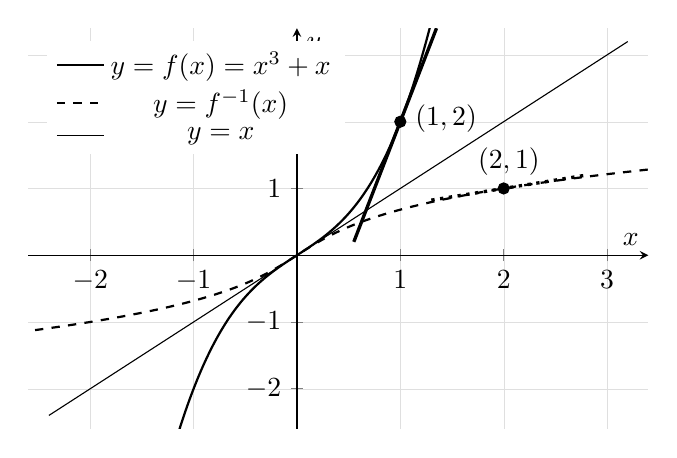
\begin{tikzpicture}
\begin{axis}[
    width=0.78\textwidth,
    height=0.55\textwidth,
    xmin=-2.6, xmax=3.4,
    ymin=-2.6, ymax=3.4,
    axis lines=middle,
    xlabel={\(x\)},
    ylabel={\(y\)},
    xtick={-2,-1,0,1,2,3},
    ytick={-2,-1,0,1,2,3},
    grid=both,
    grid style={line width=.1pt, draw=gray!25},
    legend style={draw=none, at={(0.03,0.97)}, anchor=north west}
]
\addplot[thick, domain=-1.35:1.35, samples=200] {x^3+x};
\addlegendentry{\(y=f(x)=x^3+x\)}

% inverse as reflected parametric curve
\addplot[thick, dashed, domain=-1.35:1.35, samples=200] ({x^3+x},{x});
\addlegendentry{\(y=f^{-1}(x)\)}

\addplot[thin, domain=-2.4:3.2, samples=2] {x};
\addlegendentry{\(y=x\)}

% tangent to f at (1,2): y-2=4(x-1)
\addplot[very thick, domain=0.55:1.35, samples=2] {4*x-2};

% tangent to inverse at (2,1): y-1=(1/4)(x-2)
\addplot[very thick, dotted, domain=1.3:2.8, samples=2] {0.25*x+0.5};

\addplot[only marks, mark=*] coordinates {(1,2) (2,1)};
\node[anchor=west] at (axis cs:1.05,2.05) {\((1,2)\)};
\node[anchor=south] at (axis cs:2.05,1.05) {\((2,1)\)};
\end{axis}
\end{tikzpicture}
\caption{Inverse functions are reflections across \(y=x\).  Corresponding tangent slopes are reciprocals.}
\label{fig:inverse-slopes-reciprocal}
\end{figure}

This example contains the whole rule.

If

\[
b=f(a),
\]

then

\[
f^{-1}(b)=a.
\]

The slope of \(f\) at \(a\) compares changes in output to changes in input:

\[
f'(a)\approx \frac{\Delta y}{\Delta x}.
\]

The slope of the inverse function at \(b\) compares the same small changes in the opposite direction:

\[
(f^{-1})'(b)\approx \frac{\Delta x}{\Delta y}.
\]

So the slopes should multiply to \(1\):

\[
(f^{-1})'(b)=\frac{1}{f'(a)}.
\]

Since

\[
a=f^{-1}(b),
\]

we can also write

\[
(f^{-1})'(b)=\frac{1}{f'(f^{-1}(b))}.
\]

\begin{quote}
\textbf{Derivative of an inverse function.}
Suppose \(f\) is differentiable and strictly monotone on an interval, so that \(f\) has an inverse function \(f^{-1}\).  Let

\[
b=f(a).
\]

If

\[
f'(a)\neq0,
\]

then \(f^{-1}\) is differentiable at \(b\), and

\[
\boxed{
(f^{-1})'(b)=\frac{1}{f'(a)}.
}
\]

Equivalently,

\[
\boxed{
(f^{-1})'(x)=\frac{1}{f'(f^{-1}(x))}.
}
\]
\end{quote}

The formula is easy to remember:

\[
\text{inverse slope}=\frac{1}{\text{original slope at the matching point}}.
\]

The matching point matters.  If

\[
b=f(a),
\]

then the derivative of \(f^{-1}\) at \(b\) uses the derivative of \(f\) at \(a\), not at \(b\).

\paragraph{Proof.}
Let

\[
g=f^{-1}
\]

and let

\[
b=f(a).
\]

Then

\[
g(b)=a.
\]

For \(y\neq b\), consider the difference quotient of \(g\):

\[
\frac{g(y)-g(b)}{y-b}.
\]

Since

\[
g(b)=a
\]

and

\[
y=f(g(y)),
\qquad
b=f(a),
\]

we can rewrite this as

\[
\frac{g(y)-a}{f(g(y))-f(a)}.
\]

This is the reciprocal of

\[
\frac{f(g(y))-f(a)}{g(y)-a}.
\]

As

\[
y\to b,
\]

the continuity of the inverse gives

\[
g(y)\to g(b)=a.
\]

Therefore

\[
\frac{f(g(y))-f(a)}{g(y)-a}\to f'(a).
\]

Since \(f'(a)\neq0\), we may take reciprocals in the limit:

\[
\frac{g(y)-g(b)}{y-b}\to \frac1{f'(a)}.
\]

Thus

\[
g'(b)=\frac1{f'(a)}.
\]

So

\[
\boxed{
(f^{-1})'(b)=\frac1{f'(a)}.
}
\]

\paragraph{Example.}
Let

\[
f(x)=x^3+x.
\]

Find

\[
(f^{-1})'(2).
\]

First find the input \(a\) for which

\[
f(a)=2.
\]

Since

\[
f(1)=1^3+1=2,
\]

we have

\[
a=1.
\]

Now compute

\[
f'(x)=3x^2+1.
\]

Thus

\[
f'(1)=4.
\]

Therefore

\[
\boxed{
(f^{-1})'(2)=\frac14.
}
\]

We did not need a formula for \(f^{-1}(x)\).  We only needed to know which input produced the output \(2\).

\paragraph{Example: the logarithm again.}
Let

\[
f(x)=e^x.
\]

Its inverse is

\[
f^{-1}(x)=\ln x.
\]

If

\[
x=e^a,
\]

then

\[
a=\ln x.
\]

The inverse derivative formula gives

\[
(\ln x)'=\frac1{f'(a)}.
\]

But

\[
f'(a)=e^a=x.
\]

Therefore

\[
\boxed{
\frac{d}{dx}\ln x=\frac1x.
}
\]

So the logarithm formula from the last section is one case of the inverse function rule.

\subsection{Why the nonzero derivative matters}
\label{subsec:why-nonzero-derivative-inverse}

The inverse function rule requires

\[
f'(a)\neq0.
\]

This condition is not decorative.  If the original graph has a horizontal tangent, then the inverse graph has a vertical tangent.  A vertical tangent does not have a finite derivative as a function of \(x\).

\paragraph{Example.}
Let

\[
f(x)=x^3.
\]

This function is strictly increasing, so it has an inverse:

\[
f^{-1}(x)=\sqrt[3]{x}.
\]

At

\[
a=0,
\]

we have

\[
f'(0)=3(0)^2=0.
\]

The inverse function rule would ask us to divide by \(0\), so it cannot apply.

Check directly whether

\[
g(x)=\sqrt[3]{x}
\]

has a derivative at \(0\).  The difference quotient is

\[
\frac{g(h)-g(0)}{h}
=
\frac{\sqrt[3]{h}}{h}
=
\frac1{h^{2/3}}.
\]

As \(h\to0\), this does not approach a finite number.  The inverse function is not differentiable at \(0\).

The original graph \(y=x^3\) is flat at the origin.  After reflection across \(y=x\), that flat tangent becomes vertical.

\begin{figure}[h]
\centering
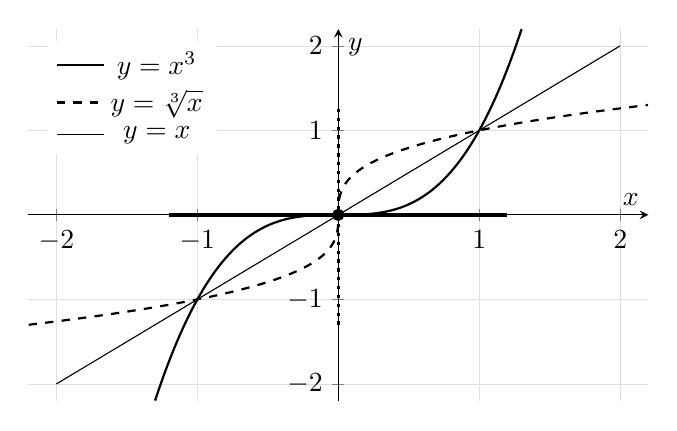
\begin{tikzpicture}
\begin{axis}[
    width=0.78\textwidth,
    height=0.52\textwidth,
    xmin=-2.2, xmax=2.2,
    ymin=-2.2, ymax=2.2,
    axis lines=middle,
    xlabel={\(x\)},
    ylabel={\(y\)},
    xtick={-2,-1,0,1,2},
    ytick={-2,-1,0,1,2},
    grid=both,
    grid style={line width=.1pt, draw=gray!25},
    legend style={draw=none, at={(0.03,0.97)}, anchor=north west}
]
\addplot[thick, domain=-1.3:1.3, samples=200] {x^3};
\addlegendentry{\(y=x^3\)}
\addplot[thick, dashed, domain=-1.3:1.3, samples=200] ({x^3},{x});
\addlegendentry{\(y=\sqrt[3]{x}\)}
\addplot[thin, domain=-2:2, samples=2] {x};
\addlegendentry{\(y=x\)}
\addplot[very thick, domain=-1.2:1.2, samples=2] {0};
\draw[very thick, dotted] (axis cs:0,-1.3) -- (axis cs:0,1.3);
\addplot[only marks, mark=*] coordinates {(0,0)};
\end{axis}
\end{tikzpicture}
\caption{The horizontal tangent to \(y=x^3\) reflects into a vertical tangent to \(y=\sqrt[3]{x}\).}
\label{fig:x-cubed-inverse-vertical}
\end{figure}

\begin{quote}
\textbf{Warning.}
A function can have an inverse even when \(f'(a)=0\).  But the inverse may fail to have a finite derivative at the corresponding point.
\end{quote}

The condition

\[
f'(a)\neq0
\]

means that, near \(a\), the original function actually changes to first order.  It does not flatten out completely.  Then the inverse has a finite local slope.

\subsection{Inverse trigonometric functions}
\label{subsec:inverse-trig-functions}

The trigonometric functions repeat.  That makes them different from \(e^x\) or \(x^3+x\).

The sine function is not one-to-one on the whole real line.  Many different angles have the same sine value.  For example,

\[
\sin\left(\frac{\pi}{6}\right)=\frac12
\]

and

\[
\sin\left(\frac{5\pi}{6}\right)=\frac12.
\]

So sine cannot have an inverse on all of \(\mathbb R\).

To reverse sine, we first choose one interval where sine is one-to-one.  The standard choice is

\[
-\frac{\pi}{2}\le x\le \frac{\pi}{2}.
\]

On this interval, sine increases from \(-1\) to \(1\).  Therefore it has an inverse function:

\[
\arcsin x.
\]

This means:

\[
\arcsin x
\]

is the angle between

\[
-\frac{\pi}{2}
\quad\text{and}\quad
\frac{\pi}{2}
\]

whose sine is \(x\).

In symbols,

\[
y=\arcsin x
\qquad\Longleftrightarrow\qquad
\sin y=x,
\quad
-\frac{\pi}{2}\le y\le\frac{\pi}{2}.
\]

\begin{figure}[h]
\centering
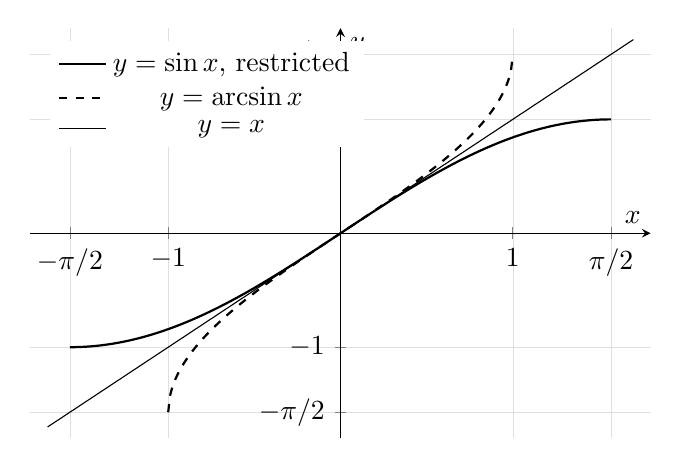
\begin{tikzpicture}
\begin{axis}[
    width=0.78\textwidth,
    height=0.56\textwidth,
    xmin=-1.8, xmax=1.8,
    ymin=-1.8, ymax=1.8,
    axis lines=middle,
    xlabel={\(x\)},
    ylabel={\(y\)},
    xtick={-1.5708,-1,0,1,1.5708},
    xticklabels={\(-\pi/2\),\(-1\),\(0\),\(1\),\(\pi/2\)},
    ytick={-1.5708,-1,0,1,1.5708},
    yticklabels={\(-\pi/2\),\(-1\),\(0\),\(1\),\(\pi/2\)},
    grid=both,
    grid style={line width=.1pt, draw=gray!25},
    legend style={draw=none, at={(0.03,0.97)}, anchor=north west}
]
\addplot[thick, domain=-1.5708:1.5708, samples=200] {sin(deg(x))};
\addlegendentry{\(y=\sin x\), restricted}

\addplot[thick, dashed, domain=-1:1, samples=200] {asin(x)*pi/180};
\addlegendentry{\(y=\arcsin x\)}

\addplot[thin, domain=-1.7:1.7, samples=2] {x};
\addlegendentry{\(y=x\)}
\end{axis}
\end{tikzpicture}
\caption{The graph of \(y=\arcsin x\) is the reflection of the restricted sine graph across \(y=x\).}
\label{fig:arcsin-reflection}
\end{figure}

The other inverse trigonometric functions are defined in the same spirit.

\[
\arccos x
\]

is the angle between \(0\) and \(\pi\) whose cosine is \(x\):

\[
y=\arccos x
\qquad\Longleftrightarrow\qquad
\cos y=x,
\quad
0\le y\le\pi.
\]

And

\[
\arctan x
\]

is the angle between \(-\pi/2\) and \(\pi/2\) whose tangent is \(x\):

\[
y=\arctan x
\qquad\Longleftrightarrow\qquad
\tan y=x,
\quad
-\frac{\pi}{2}< y<\frac{\pi}{2}.
\]

\begin{quote}
\textbf{Notation warning.}
Some books write

\[
\sin^{-1}x
\]

for

\[
\arcsin x.
\]

This does not mean

\[
\frac1{\sin x}.
\]

To avoid confusion, we will use \(\arcsin x\), \(\arccos x\), and \(\arctan x\).
\end{quote}

\subsection{The derivative of \texorpdfstring{\(\arcsin x\)}{arcsin x}}
\label{subsec:derivative-arcsin}

Let

\[
y=\arcsin x.
\]

Then

\[
\sin y=x,
\]

where

\[
-\frac{\pi}{2}\le y\le \frac{\pi}{2}.
\]

Differentiate both sides with respect to \(x\).  Since \(y\) depends on \(x\), the left side uses implicit differentiation:

\[
\cos y\frac{dy}{dx}=1.
\]

Therefore

\[
\frac{dy}{dx}=\frac1{\cos y}.
\]

Now rewrite \(\cos y\) in terms of \(x\).  Since

\[
\sin y=x,
\]

we have

\[
\cos^2y=1-\sin^2y=1-x^2.
\]

On the interval

\[
-\frac{\pi}{2}\le y\le \frac{\pi}{2},
\]

cosine is nonnegative.  Therefore

\[
\cos y=\sqrt{1-x^2}.
\]

Thus

\[
\boxed{
\frac{d}{dx}\arcsin x=\frac1{\sqrt{1-x^2}},
\qquad -1<x<1.
}
\]

The derivative is not finite at \(x=1\) or \(x=-1\).  Geometrically, the graph of \(\arcsin x\) has vertical tangents at the endpoints.

\paragraph{Example.}
Differentiate

\[
F(x)=\arcsin(x^2).
\]

Let

\[
u=x^2.
\]

Then

\[
F(x)=\arcsin u.
\]

Using the chain rule,

\[
F'(x)=\frac{1}{\sqrt{1-u^2}}u'.
\]

Since

\[
u'=2x,
\]

we get

\[
\boxed{
F'(x)=\frac{2x}{\sqrt{1-x^4}}.
}
\]

This derivative is valid where

\[
-1<x^2<1,
\]

so

\[
-1<x<1.
\]

\subsection{The derivatives of \texorpdfstring{\(\arccos x\)}{arccos x} and \texorpdfstring{\(\arctan x\)}{arctan x}}
\label{subsec:derivatives-arccos-arctan}

For arccosine, let

\[
y=\arccos x.
\]

Then

\[
\cos y=x,
\qquad
0\le y\le \pi.
\]

Differentiate:

\[
-\sin y\frac{dy}{dx}=1.
\]

So

\[
\frac{dy}{dx}=-\frac1{\sin y}.
\]

Since

\[
\cos y=x,
\]

we have

\[
\sin^2y=1-x^2.
\]

On \(0\le y\le\pi\), sine is nonnegative, so

\[
\sin y=\sqrt{1-x^2}.
\]

Therefore

\[
\boxed{
\frac{d}{dx}\arccos x=-\frac1{\sqrt{1-x^2}},
\qquad -1<x<1.
}
\]

The minus sign makes sense: \(\arccos x\) decreases as \(x\) increases.

For arctangent, let

\[
y=\arctan x.
\]

Then

\[
\tan y=x,
\qquad
-\frac{\pi}{2}<y<\frac{\pi}{2}.
\]

Differentiate:

\[
\sec^2 y\frac{dy}{dx}=1.
\]

So

\[
\frac{dy}{dx}=\frac1{\sec^2y}.
\]

Using the identity

\[
\sec^2 y=1+\tan^2y,
\]

and

\[
\tan y=x,
\]

we get

\[
\sec^2y=1+x^2.
\]

Therefore

\[
\boxed{
\frac{d}{dx}\arctan x=\frac1{1+x^2}.
}
\]

This derivative is defined for every real \(x\).

\paragraph{Example.}
Differentiate

\[
G(x)=\arctan(3x^2).
\]

Let

\[
u=3x^2.
\]

Then

\[
G(x)=\arctan u.
\]

By the chain rule,

\[
G'(x)=\frac{u'}{1+u^2}.
\]

Since

\[
u'=6x,
\]

we get

\[
\boxed{
G'(x)=\frac{6x}{1+9x^4}.
}
\]

\paragraph{Example.}
Find the tangent line to

\[
y=\arctan x
\]

at

\[
x=1.
\]

First,

\[
\arctan 1=\frac{\pi}{4}.
\]

The slope is

\[
y'(1)=\frac1{1+1^2}=\frac12.
\]

Therefore the tangent line is

\[
\boxed{
y-\frac{\pi}{4}=\frac12(x-1).
}
\]

\subsection{A table of inverse trigonometric derivatives}
\label{subsec:inverse-trig-derivative-table}

The three most important inverse trigonometric derivatives are

\[
\boxed{
\begin{array}{c|c}
\text{function} & \text{derivative} \\ \hline
\arcsin x & \dfrac1{\sqrt{1-x^2}} \\[8pt]
\arccos x & -\dfrac1{\sqrt{1-x^2}} \\[8pt]
\arctan x & \dfrac1{1+x^2}
\end{array}
}
\]

The remaining inverse trigonometric derivatives follow from the same method.  With the usual choices of inverse branches,

\[
\boxed{
\begin{array}{c|c}
\text{function} & \text{derivative} \\ \hline
\operatorname{arccot} x & -\dfrac1{1+x^2} \\[8pt]
\operatorname{arcsec} x & \dfrac1{|x|\sqrt{x^2-1}} \\[8pt]
\operatorname{arccsc} x & -\dfrac1{|x|\sqrt{x^2-1}}
\end{array}
}
\]

The absolute value in the arcsecant and arccosecant formulas comes from the branch choices and the sign of the trigonometric functions on those branches.

\subsection{Inverse trigonometric derivatives as an integration preview}
\label{subsec:inverse-trig-integration-preview}

For now, these formulas help us differentiate.  Later, when we reverse derivatives, they will become integration patterns.

The formula

\[
\frac{d}{dx}\arcsin x=\frac1{\sqrt{1-x^2}}
\]

will be read backward as

\[
\int \frac{dx}{\sqrt{1-x^2}}=\arcsin x+C.
\]

The formula

\[
\frac{d}{dx}\arctan x=\frac1{1+x^2}
\]

will be read backward as

\[
\int \frac{dx}{1+x^2}=\arctan x+C.
\]

So the shapes

\[
\frac1{\sqrt{1-x^2}}
\qquad\text{and}\qquad
\frac1{1+x^2}
\]

are worth remembering.  They are not random fractions.  They are the derivative fingerprints of inverse trigonometric functions.

\paragraph{Example.}
Differentiate

\[
H(x)=x\arctan x.
\]

Use the product rule:

\[
H'(x)=1\cdot\arctan x+x\cdot\frac1{1+x^2}.
\]

Thus

\[
\boxed{
H'(x)=\arctan x+\frac{x}{1+x^2}.
}
\]

Later, this same computation will help us integrate \(\arctan x\).  Many integration techniques are differentiation rules read backward, with more strategy required.

Inverse functions reverse input and output.  The next section returns to powers, where the exponent need not be an integer.  That extension also depends on reversing functions, because real powers are most naturally handled with logarithms.

\section{General power rule and hyperbolic functions}
\label{sec:general-power-rule-hyperbolic-functions}

The power rule first appeared for positive integer powers:

\[
\frac{d}{dx}x^n=nx^{n-1}.
\]

Then negative powers came from the reciprocal rule, and fractional-looking powers appeared through roots.  But the formula is larger than all of those cases.

It works for any real exponent, as long as the function is defined and differentiable.

The logarithm gives the cleanest proof.

\subsection{The derivative of \texorpdfstring{\(x^r\)}{x to the r}}
\label{subsec:derivative-x-to-r}

Suppose

\[
y=x^\pi,
\qquad x>0.
\]

This is not a polynomial.  The exponent is not an integer.  But logarithms turn powers into products.

Take natural logarithms:

\[
\ln y=\ln(x^\pi).
\]

Using the logarithm rule,

\[
\ln y=\pi\ln x.
\]

Differentiate both sides with respect to \(x\).  The left side uses the chain rule:

\[
\frac1y\frac{dy}{dx}=\pi\frac1x.
\]

So

\[
\frac{dy}{dx}=y\frac{\pi}{x}.
\]

Since

\[
y=x^\pi,
\]

we get

\[
\frac{dy}{dx}=x^\pi\frac{\pi}{x}.
\]

Therefore

\[
\boxed{
\frac{d}{dx}x^\pi=\pi x^{\pi-1},
\qquad x>0.
}
\]

Nothing special about \(\pi\) was used.  The same argument works for any real exponent.

\begin{quote}
\textbf{General Power Rule.}
For any fixed real number \(r\),

\[
\boxed{
\frac{d}{dx}x^r=rx^{r-1},
\qquad x>0.
}
\]

When \(x^r\) is defined on a larger domain, the same formula holds at points where the derivative exists.  The logarithmic proof above applies directly on \(x>0\).
\end{quote}

\paragraph{Proof.}
Let

\[
y=x^r,
\qquad x>0.
\]

Take logarithms:

\[
\ln y=r\ln x.
\]

Differentiate both sides:

\[
\frac1y y'=\frac r x.
\]

Multiply by \(y\):

\[
y'=y\frac r x.
\]

Since

\[
y=x^r,
\]

we have

\[
y'=x^r\frac r x=rx^{r-1}.
\]

Thus

\[
\boxed{
\frac{d}{dx}x^r=rx^{r-1}.
}
\]

\paragraph{Example.}
Differentiate

\[
f(x)=x^{\sqrt2},
\qquad x>0.
\]

Using the general power rule,

\[
\boxed{
f'(x)=\sqrt2\,x^{\sqrt2-1}.
}
\]

\paragraph{Example.}
Differentiate

\[
g(x)=(1+x^2)^{5/2}.
\]

Let

\[
u=1+x^2.
\]

Then

\[
g(x)=u^{5/2}.
\]

By the general power rule and the chain rule,

\[
g'(x)=\frac52 u^{3/2}u'.
\]

Since

\[
u'=2x,
\]

we get

\[
\boxed{
g'(x)=5x(1+x^2)^{3/2}.
}
\]

\paragraph{Example.}
Differentiate

\[
h(x)=\sqrt[3]{x}.
\]

For \(x\neq0\),

\[
h(x)=x^{1/3}.
\]

So

\[
h'(x)=\frac13x^{-2/3}.
\]

Thus

\[
\boxed{
h'(x)=\frac1{3x^{2/3}},
\qquad x\neq0.
}
\]

At \(x=0\), the function is defined, but the derivative is not finite.  Indeed,

\[
\frac{h(0+k)-h(0)}{k}
=
\frac{\sqrt[3]{k}}{k}
=
\frac1{k^{2/3}},
\]

which becomes unbounded as \(k\to0\).

\begin{quote}
\textbf{Warning at \(x=0\).}
The formula

\[
\frac{d}{dx}x^r=rx^{r-1}
\]

does not automatically settle what happens at \(x=0\).  The function may be defined there while the derivative fails to exist, as with \(x^{1/3}\).  Always check the domain and the point.
\end{quote}

\subsection{Hyperbolic sine and cosine}
\label{subsec:hyperbolic-sine-cosine}

The exponential function has two natural halves: an even half and an odd half.

The even half is

\[
\cosh x=\frac{e^x+e^{-x}}2.
\]

The odd half is

\[
\sinh x=\frac{e^x-e^{-x}}2.
\]

These are called the \emph{hyperbolic cosine} and \emph{hyperbolic sine}.

The names look trigonometric, but the definitions are exponential.  That makes their derivatives immediate.

Differentiate \(\sinh x\):

\[
\frac{d}{dx}\sinh x
=
\frac{d}{dx}\left(\frac{e^x-e^{-x}}2\right).
\]

Since

\[
\frac{d}{dx}e^{-x}=-e^{-x},
\]

we get

\[
\frac{d}{dx}\sinh x
=
\frac{e^x+e^{-x}}2.
\]

Therefore

\[
\boxed{
\frac{d}{dx}\sinh x=\cosh x.
}
\]

Now differentiate \(\cosh x\):

\[
\frac{d}{dx}\cosh x
=
\frac{d}{dx}\left(\frac{e^x+e^{-x}}2\right)
=
\frac{e^x-e^{-x}}2.
\]

Therefore

\[
\boxed{
\frac{d}{dx}\cosh x=\sinh x.
}
\]

Compare this with sine and cosine:

\[
(\sin x)'=\cos x,
\qquad
(\cos x)'=-\sin x.
\]

For hyperbolic functions, the minus sign disappears:

\[
(\sinh x)'=\cosh x,
\qquad
(\cosh x)'=\sinh x.
\]

\begin{figure}[h]
\centering
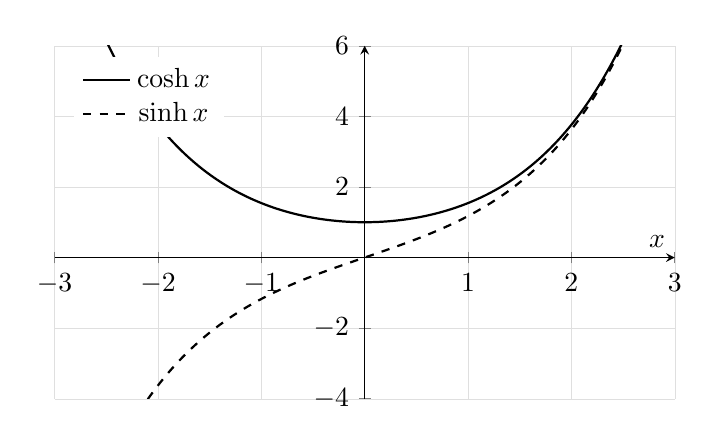
\begin{tikzpicture}
\begin{axis}[
    width=0.78\textwidth,
    height=0.50\textwidth,
    xmin=-3, xmax=3,
    ymin=-4, ymax=6,
    axis lines=middle,
    xlabel={\(x\)},
    ylabel={},
    xtick={-3,-2,-1,0,1,2,3},
    ytick={-4,-2,0,2,4,6},
    grid=both,
    grid style={line width=.1pt, draw=gray!25},
    legend style={draw=none, at={(0.03,0.97)}, anchor=north west}
]
\addplot[thick, domain=-3:3, samples=200] {cosh(x)};
\addlegendentry{\(\cosh x\)}
\addplot[thick, dashed, domain=-3:3, samples=200] {sinh(x)};
\addlegendentry{\(\sinh x\)}
\end{axis}
\end{tikzpicture}
\caption{The function \(\cosh x\) is even, while \(\sinh x\) is odd.}
\label{fig:sinh-cosh-graphs}
\end{figure}

These functions also recombine to give exponentials:

\[
\cosh x+\sinh x=e^x,
\]

because

\[
\frac{e^x+e^{-x}}2+\frac{e^x-e^{-x}}2=e^x.
\]

Similarly,

\[
\cosh x-\sinh x=e^{-x}.
\]

So hyperbolic functions are not new mysteries.  They are a useful way to package exponentials symmetrically.

\paragraph{Example.}
Differentiate

\[
y=\cosh(3x^2).
\]

Let

\[
u=3x^2.
\]

Then

\[
y=\cosh u.
\]

By the chain rule,

\[
y'=\sinh u\cdot u'.
\]

Since

\[
u'=6x,
\]

we get

\[
\boxed{
y'=6x\sinh(3x^2).
}
\]

\paragraph{Example.}
Differentiate

\[
y=e^x\cosh x.
\]

Use the product rule:

\[
y'=e^x\cosh x+e^x\sinh x.
\]

Factor:

\[
y'=e^x(\cosh x+\sinh x).
\]

Since

\[
\cosh x+\sinh x=e^x,
\]

we get

\[
\boxed{
y'=e^{2x}.
}
\]

This also follows from rewriting the original function:

\[
e^x\cosh x
=
e^x\frac{e^x+e^{-x}}2
=
\frac{e^{2x}+1}{2}.
\]

Then

\[
\frac{d}{dx}\left(\frac{e^{2x}+1}{2}\right)=e^{2x}.
\]

\subsection{Hyperbolic identities}
\label{subsec:hyperbolic-identities}

The ordinary trigonometric functions satisfy

\[
\cos^2 x+\sin^2 x=1.
\]

The hyperbolic functions satisfy a similar identity, but with a minus sign:

\[
\boxed{
\cosh^2 x-\sinh^2 x=1.
}
\]

To prove it, use the definitions:

\[
\cosh^2x-\sinh^2x
=
\left(\frac{e^x+e^{-x}}2\right)^2
-
\left(\frac{e^x-e^{-x}}2\right)^2.
\]

Use the difference of squares:

\[
A^2-B^2=(A-B)(A+B).
\]

Here

\[
A=\frac{e^x+e^{-x}}2,
\qquad
B=\frac{e^x-e^{-x}}2.
\]

Then

\[
A-B=e^{-x},
\qquad
A+B=e^x.
\]

Therefore

\[
\cosh^2x-\sinh^2x=e^{-x}e^x=1.
\]

This identity explains the word \emph{hyperbolic}.  If

\[
X=\cosh t,
\qquad
Y=\sinh t,
\]

then

\[
X^2-Y^2=1.
\]

So the point

\[
(\cosh t,\sinh t)
\]

lies on the right branch of the hyperbola

\[
X^2-Y^2=1.
\]

\begin{figure}[h]
\centering
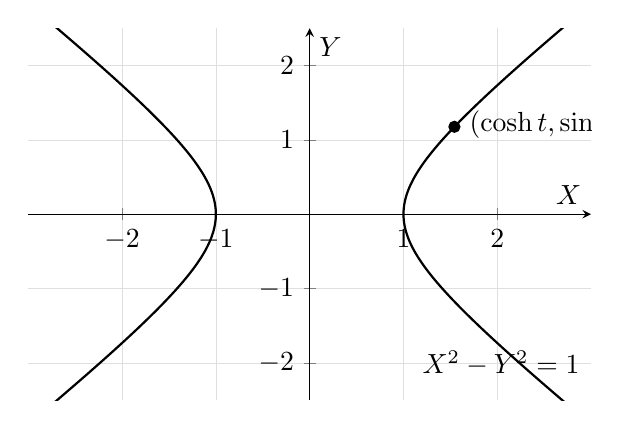
\begin{tikzpicture}
\begin{axis}[
    width=0.72\textwidth,
    height=0.52\textwidth,
    xmin=-3, xmax=3,
    ymin=-2.5, ymax=2.5,
    axis lines=middle,
    xlabel={\(X\)},
    ylabel={\(Y\)},
    xtick={-2,-1,0,1,2},
    ytick={-2,-1,0,1,2},
    grid=both,
    grid style={line width=.1pt, draw=gray!25}
]
% right branch: X = cosh t, Y = sinh t
\addplot[thick, domain=-1.8:1.8, samples=200] ({cosh(x)},{sinh(x)});
% left branch
\addplot[thick, domain=-1.8:1.8, samples=200] ({-cosh(x)},{sinh(x)});
\addplot[only marks, mark=*] coordinates {(1.543,1.175)};
\node[anchor=west] at (axis cs:1.6,1.2) {\((\cosh t,\sinh t)\)};
\node[anchor=west] at (axis cs:1.1,-2.0) {\(X^2-Y^2=1\)};
\end{axis}
\end{tikzpicture}
\caption{The parametrization \(X=\cosh t\), \(Y=\sinh t\) lies on the hyperbola \(X^2-Y^2=1\).}
\label{fig:hyperbola-cosh-sinh}
\end{figure}

This is parallel to the circular parametrization

\[
X=\cos t,
\qquad
Y=\sin t,
\]

which satisfies

\[
X^2+Y^2=1.
\]

Circular functions live on the circle

\[
X^2+Y^2=1.
\]

Hyperbolic functions live on the hyperbola

\[
X^2-Y^2=1.
\]

The addition formulas also resemble the trigonometric ones:

\[
\boxed{
\sinh(x+y)=\sinh x\cosh y+\cosh x\sinh y,
}
\]

and

\[
\boxed{
\cosh(x+y)=\cosh x\cosh y+\sinh x\sinh y.
}
\]

The signs are different from the circular formulas because the identity is

\[
\cosh^2x-\sinh^2x=1
\]

instead of

\[
\cos^2x+\sin^2x=1.
\]

\subsection{Hyperbolic tangent and its derivative}
\label{subsec:hyperbolic-tangent}

Define

\[
\tanh x=\frac{\sinh x}{\cosh x}.
\]

Using the quotient rule,

\[
\frac{d}{dx}\tanh x
=
\frac{\cosh x(\cosh x)-\sinh x(\sinh x)}{\cosh^2x}.
\]

The numerator is

\[
\cosh^2x-\sinh^2x=1.
\]

Therefore

\[
\boxed{
\frac{d}{dx}\tanh x=\frac1{\cosh^2x}.
}
\]

We write

\[
\operatorname{sech}x=\frac1{\cosh x}.
\]

So

\[
\boxed{
\frac{d}{dx}\tanh x=\operatorname{sech}^2x.
}
\]

This looks like

\[
\frac{d}{dx}\tan x=\sec^2x,
\]

and that is not an accident.  The hyperbolic identities and trigonometric identities run in parallel, with small sign changes.

\paragraph{Example.}
Differentiate

\[
y=\tanh(\ln x),
\qquad x>0.
\]

Let

\[
u=\ln x.
\]

Then

\[
y=\tanh u.
\]

By the chain rule,

\[
y'=\operatorname{sech}^2u\cdot u'.
\]

Since

\[
u'=\frac1x,
\]

we get

\[
\boxed{
y'=\frac{\operatorname{sech}^2(\ln x)}{x}.
}
\]

\subsection{Why hyperbolic functions appear in hanging cables}
\label{subsec:hanging-cables-hyperbolic-functions}

A hanging cable does not form a parabola.  It forms a \emph{catenary}, whose basic shape is

\[
y=a\cosh\left(\frac{x}{a}\right).
\]

The full physics belongs later, but the main reason can already be checked with derivatives.

Suppose a cable hangs under its own weight.  Place the lowest point at the center.  Let \(s(x)\) be the arc length of the cable from the lowest point to the point with horizontal coordinate \(x\).

The slope of the cable is related to how much cable is hanging between the center and that point.  A standard force-balance model leads to

\[
y'=\frac{s}{a},
\]

where \(a>0\) is a constant depending on the horizontal tension and the weight per unit length.

Differentiate both sides with respect to \(x\):

\[
y''=\frac1a\frac{ds}{dx}.
\]

The derivative of arc length with respect to \(x\) is

\[
\frac{ds}{dx}=\sqrt{1+(y')^2}.
\]

So the shape satisfies the differential equation

\[
\boxed{
y''=\frac1a\sqrt{1+(y')^2}.
}
\]

Now check that

\[
y=a\cosh\left(\frac{x}{a}\right)
\]

solves it.

First derivative:

\[
y'
=
a\sinh\left(\frac{x}{a}\right)\cdot \frac1a
=
\sinh\left(\frac{x}{a}\right).
\]

Second derivative:

\[
y''
=
\cosh\left(\frac{x}{a}\right)\cdot\frac1a
=
\frac1a\cosh\left(\frac{x}{a}\right).
\]

The right side of the differential equation is

\[
\frac1a\sqrt{1+(y')^2}
=
\frac1a\sqrt{1+\sinh^2\left(\frac{x}{a}\right)}.
\]

Using

\[
\cosh^2 u-\sinh^2 u=1,
\]

we have

\[
1+\sinh^2u=\cosh^2u.
\]

Since \(\cosh u>0\),

\[
\sqrt{1+\sinh^2u}=\cosh u.
\]

Therefore

\[
\frac1a\sqrt{1+(y')^2}
=
\frac1a\cosh\left(\frac{x}{a}\right)
=
y''.
\]

So

\[
\boxed{
y=a\cosh\left(\frac{x}{a}\right)
}
\]

has exactly the derivative behavior required by the cable model.

\begin{figure}[h]
\centering
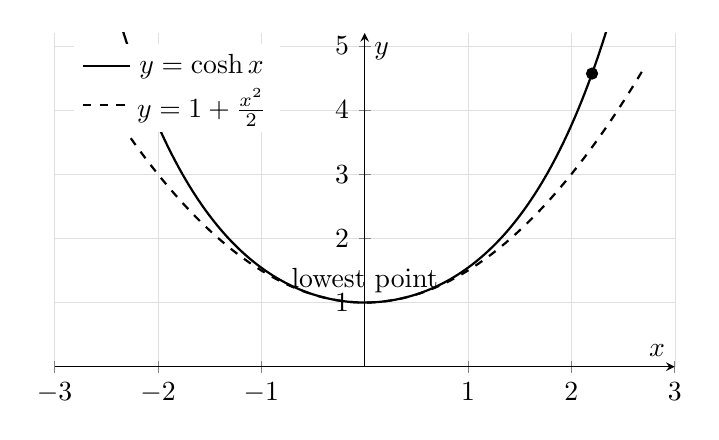
\begin{tikzpicture}
\begin{axis}[
    width=0.78\textwidth,
    height=0.48\textwidth,
    xmin=-3, xmax=3,
    ymin=0, ymax=5.2,
    axis lines=middle,
    xlabel={\(x\)},
    ylabel={\(y\)},
    xtick={-3,-2,-1,0,1,2,3},
    ytick={0,1,2,3,4,5},
    grid=both,
    grid style={line width=.1pt, draw=gray!25},
    legend style={draw=none, at={(0.03,0.97)}, anchor=north west}
]
\addplot[thick, domain=-2.7:2.7, samples=200] {cosh(x)};
\addlegendentry{\(y=\cosh x\)}
\addplot[thick, dashed, domain=-2.7:2.7, samples=200] {1+x^2/2};
\addlegendentry{\(y=1+\frac{x^2}{2}\)}
\addplot[only marks, mark=*, samples at={-2.2, 2.2}] {cosh(x)};
\node[anchor=south] at (axis cs:0,1) {lowest point};
\end{axis}
\end{tikzpicture}
\caption{Near the lowest point, a catenary resembles a parabola.  Farther away, the hyperbolic cosine shape rises differently.}
\label{fig:catenary-cosh}
\end{figure}

This is a good preview of differential equations.  A physical law can describe a curve by a relation among its derivatives.  Solving the law means finding a function with exactly that derivative behavior.

Hyperbolic functions are useful because they are built from exponentials and have simple derivative cycles:

\[
(\sinh x)'=\cosh x,
\qquad
(\cosh x)'=\sinh x.
\]

They are not just extra names.  They package the functions that naturally solve some laws of growth, balance, and shape.

\subsection{The derivative table at the end of Chapter 5}
\label{subsec:chapter-5-derivative-table-end}

Chapter 5 has built a large but organized table of derivatives:

\[
\boxed{
\begin{array}{c|c}
\text{function} & \text{derivative} \\ \hline
x^r & rx^{r-1} \\[3pt]
e^x & e^x \\[3pt]
a^x & (\ln a)a^x \\[3pt]
\ln x & \dfrac1x \\[8pt]
\sin x & \cos x \\[3pt]
\cos x & -\sin x \\[3pt]
\tan x & \sec^2x \\[3pt]
\arcsin x & \dfrac1{\sqrt{1-x^2}} \\[8pt]
\arctan x & \dfrac1{1+x^2} \\[8pt]
\sinh x & \cosh x \\[3pt]
\cosh x & \sinh x
\end{array}
}
\]

The rules behind the table are just as important as the table itself:

\[
\text{sum rule, product rule, quotient rule, chain rule, inverse rule.}
\]

These rules let us differentiate complicated functions by reading how they are built.

But derivatives are not only for computing more derivatives.  They reveal the shape of a function.

If

\[
f'(x)>0,
\]

the function should be increasing.  If

\[
f'(x)<0,
\]

it should be decreasing.  If

\[
f'(x)=0,
\]

something special may happen: a peak, a valley, or perhaps only a pause.

The next chapter asks how much of a graph can be understood from its derivative.

\section{Warning examples}
\label{sec:warning-examples-differentiation-rules}

This chapter has given us speed.  We no longer need to return to the limit definition every time we differentiate.  We have rules.

That speed is useful, but it also creates a danger.  A rule that is remembered only as a symbol can be used in the wrong place.

The safest way to use derivative rules is to keep asking:

\[
\text{How was this function built?}
\]

A sum, a product, a quotient, a composition, and an inverse are different constructions.  Their derivatives are different because their changes are different.

\subsection{The product rule is not \texorpdfstring{\((fg)'=f'g'\)}{(fg)'=f'g'}}
\label{subsec:product-rule-not-product-of-derivatives}

A common mistake is to guess that the derivative of a product is the product of the derivatives:

\[
(fg)' \stackrel{\text{wrong}}{=} f'g'.
\]

This is false.

Take the simplest possible example:

\[
f(x)=x,
\qquad
g(x)=x.
\]

Then

\[
f(x)g(x)=x^2.
\]

So

\[
(fg)'(x)=2x.
\]

But

\[
f'(x)g'(x)=1\cdot1=1.
\]

These are not the same.  For example, at \(x=3\),

\[
(fg)'(3)=6,
\qquad
f'(3)g'(3)=1.
\]

The correct rule is

\[
\boxed{
(fg)'=f'g+fg'.
}
\]

This rule has a geometric picture visualization.  If a rectangle has side lengths \(f(x)\) and \(g(x)\), then its area is

\[
A(x)=f(x)g(x).
\]

When \(x\) changes a little, both sides may change.  The new area comes from two first-order strips:

\[
f'(x)g(x)\Delta x
\qquad\text{and}\qquad
f(x)g'(x)\Delta x.
\]

That is why two terms appear.

\begin{figure}[h]
\centering
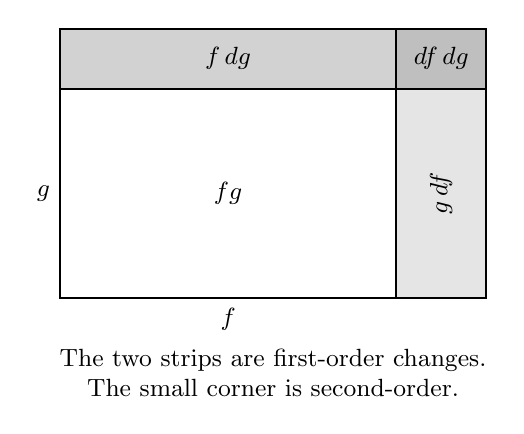
\begin{tikzpicture}[scale=0.95, every node/.style={font=\small}]
  % original rectangle
  \draw[thick] (0,0) rectangle (4.5,2.8);
  \node at (2.25,1.4) {\(fg\)};
  \node[below] at (2.25,0) {\(f\)};
  \node[left] at (0,1.4) {\(g\)};

  % right strip (g df)
  \fill[gray!20] (4.5,0) rectangle (5.7,2.8);
  \draw[thick] (4.5,0) rectangle (5.7,2.8);
  \node[rotate=90] at (5.1,1.4) {\(g\,df\)};

  % top strip (f dg)
  \fill[gray!35] (0,2.8) rectangle (4.5,3.6);
  \draw[thick] (0,2.8) rectangle (4.5,3.6);
  \node at (2.25,3.2) {\(f\,dg\)};

  % small corner (df dg)
  \fill[gray!50] (4.5,2.8) rectangle (5.7,3.6);
  \draw[thick] (4.5,2.8) rectangle (5.7,3.6);
  \node at (5.1,3.2) {\(df\,dg\)}; % Moved inside the rectangle

  % explanatory text
  \node[align=center] at (2.85,-1.0)
  {The two strips are first-order changes.\\
  The small corner is second-order.};
\end{tikzpicture}
\caption{A changing product has two first-order contributions, not one.}
\label{fig:product-rule-warning-strips}
\end{figure}

In differential notation,

\[
d(fg)
=
(f+df)(g+dg)-fg.
\]

Expanding,

\[
d(fg)=f\,dg+g\,df+df\,dg.
\]

The term \(df\,dg\) is much smaller than the first-order terms when the change is tiny.  Dividing by \(dx\) and passing to the limit gives

\[
(fg)'=fg'+gf'.
\]

The false rule \(f'g'\) forgets the original sizes \(f\) and \(g\).  But the original sizes matter.  A small change in the width of a large rectangle adds more area than the same change in the width of a small rectangle.

\paragraph{Another quick test.}
Let

\[
f(x)=x^2,
\qquad
g(x)=\sin x.
\]

Then

\[
(fg)'=2x\sin x+x^2\cos x.
\]

But

\[
f'g'=(2x)(\cos x)=2x\cos x.
\]

The false rule loses the term \(2x\sin x\) and changes the other term.  It is not a small error.  It is a different derivative.

\begin{quote}
\textbf{Product warning.}
Do not multiply derivatives.  Differentiate the product by letting each factor change once:

\[
\boxed{
(fg)'=f'g+fg'.
}
\]
\end{quote}

\subsection{The chain rule needs the order of composition}
\label{subsec:chain-rule-composition-order-warning}

The chain rule is a rule for functions built in layers.  The order of the layers matters.

Let

\[
f(u)=\sin u,
\qquad
g(x)=x^2.
\]

There are two different composites:

\[
f(g(x))=\sin(x^2),
\]

and

\[
g(f(x))=(\sin x)^2.
\]

They use the same two functions, but in different orders.

\begin{figure}[h]
\centering
\begin{tikzpicture}[every node/.style={font=\small}, node distance=2.6cm]
  % first chain
  \node (x1) at (0,1.3) {\(\boxed{x}\)};
  \node (g1) at (2.8,1.3) {\(\boxed{x^2}\)};
  \node (f1) at (5.8,1.3) {\(\boxed{\sin(x^2)}\)};
  \draw[->, thick] (x1) -- node[above] {\(g\)} (g1);
  \draw[->, thick] (g1) -- node[above] {\(f\)} (f1);

  % second chain
  \node (x2) at (0,-1.3) {\(\boxed{x}\)};
  \node (f2) at (2.8,-1.3) {\(\boxed{\sin x}\)};
  \node (g2) at (5.8,-1.3) {\(\boxed{(\sin x)^2}\)};
  \draw[->, thick] (x2) -- node[above] {\(f\)} (f2);
  \draw[->, thick] (f2) -- node[above] {\(g\)} (g2);

  \node at (8.2,1.3) {\(f\circ g\)};
  \node at (8.2,-1.3) {\(g\circ f\)};
\end{tikzpicture}
\caption{The same two functions in different orders produce different chains.}
\label{fig:chain-rule-order-warning}
\end{figure}

Differentiate the first one:

\[
\frac{d}{dx}\sin(x^2)
=
\cos(x^2)\cdot 2x.
\]

So

\[
\boxed{
\frac{d}{dx}\sin(x^2)=2x\cos(x^2).
}
\]

Differentiate the second one:

\[
\frac{d}{dx}(\sin x)^2
=
2\sin x\cdot\cos x.
\]

So

\[
\boxed{
\frac{d}{dx}(\sin x)^2=2\sin x\cos x.
}
\]

These are not the same derivative because the original functions are not the same function.

The chain rule says

\[
\boxed{
\frac{d}{dx}f(g(x))=f'(g(x))g'(x).
}
\]

The outside derivative is evaluated at the inside value.  That detail is easy to miss.

For

\[
y=\sin(x^2),
\]

the outside function is

\[
f(u)=\sin u.
\]

Its derivative is

\[
f'(u)=\cos u.
\]

At the current inside value

\[
u=x^2,
\]

this becomes

\[
\cos(x^2).
\]

Then we multiply by the inside derivative

\[
\frac{d}{dx}(x^2)=2x.
\]

So the derivative is

\[
2x\cos(x^2).
\]

\paragraph{A wrong answer and why it is wrong.}
For

\[
y=\sin(x^2),
\]

a common wrong answer is

\[
2\sin x\cos x.
\]

But that is the derivative of

\[
(\sin x)^2,
\]

not of

\[
\sin(x^2).
\]

The mistake changed the order of construction.

\begin{quote}
\textbf{Chain warning.}
Differentiate from the outside inward, but keep the layers in their original order.

\[
\text{outside derivative at the inside value}
\quad \times \quad
\text{inside derivative}.
\]
\end{quote}

\subsection{An inverse can fail to be differentiable}
\label{subsec:inverse-can-fail-differentiable-warning}

The inverse derivative formula says:

\[
(f^{-1})'(b)=\frac1{f'(a)}
\qquad
\text{when } b=f(a).
\]

But this formula has a condition:

\[
f'(a)\neq0.
\]

The condition matters.

Let

\[
f(x)=x^3.
\]

This function is strictly increasing, so it has an inverse:

\[
f^{-1}(x)=\sqrt[3]{x}.
\]

At

\[
a=0,
\]

we have

\[
f'(x)=3x^2,
\]

so

\[
f'(0)=0.
\]

The inverse derivative formula would require division by zero.  That is already a warning.

Check directly.  Let

\[
g(x)=\sqrt[3]{x}.
\]

Then

\[
g(0)=0.
\]

The difference quotient at \(0\) is

\[
\frac{g(0+h)-g(0)}{h}
=
\frac{\sqrt[3]{h}}{h}.
\]

For \(h\neq0\),

\[
\frac{\sqrt[3]{h}}{h}
=
\frac{1}{h^{2/3}}.
\]

As

\[
h\to0,
\]

this quotient becomes unbounded.  It does not approach a finite number.  Therefore

\[
g'(0)
\]

does not exist as a finite derivative.

The geometry explains the algebra.  The graph of \(y=x^3\) has a horizontal tangent at the origin.  Reflecting across the line \(y=x\) turns that horizontal tangent into a vertical tangent.  A vertical tangent does not have a finite slope as a function \(y=g(x)\).

\begin{quote}
\textbf{Inverse warning.}
An inverse may exist even when the inverse derivative formula cannot be used.  If the original tangent is horizontal, the inverse tangent may be vertical.
\end{quote}

The condition

\[
f'(a)\neq0
\]

does not say that \(f\) must be steep.  It says that, to first order, \(f\) must actually change.  If the original function flattens completely at a point, reversing it may create an infinite slope.

\subsection{A rule checklist}
\label{subsec:derivative-rule-checklist}

When a derivative gets complicated, do not start by writing symbols quickly.  Start by reading the structure.

\[
\begin{array}{c|c|c}
\textbf{structure} & \textbf{example} & \textbf{rule to use} \\ \hline
\text{sum} & x^2+\sin x & \text{sum rule} \\[2pt]
\text{constant multiple} & 7e^x & \text{constant multiple rule} \\[2pt]
\text{product} & x^2\ln x & \text{product rule} \\[2pt]
\text{quotient} & \dfrac{\sin x}{1+x^2} & \text{quotient rule} \\[10pt]
\text{composition} & \sin(x^2) & \text{chain rule} \\[2pt]
\text{implicit relation} & x^2+y^2=25 & \text{implicit differentiation} \\[2pt]
\text{inverse} & \arctan x & \text{inverse function rule}
\end{array}
\]

The most useful questions are:

\[
\begin{array}{l}
\text{1. Is this built by addition, multiplication, division, or composition?}\\
\text{2. If it is a composition, what is the inside function?}\\
\text{3. If it is a product or quotient, have all factors been differentiated correctly?}\\
\text{4. If it is an inverse or logarithm, are the domain conditions satisfied?}\\
\text{5. Does the final answer have the right rough behavior and units?}
\end{array}
\]

A derivative formula is not only an answer.  It is a record of how the function was built.

\section{Chapter review and discovery problems}
\label{sec:chapter-review-differentiation-rules}

Chapter 4 defined the derivative:

\[
f'(a)=\lim_{h\to0}\frac{f(a+h)-f(a)}{h}.
\]

That definition gave meaning, but it was too slow for everyday use.

Chapter 5 built a working language.  We learned how derivatives behave under algebra, composition, implicit relations, inverse functions, and the elementary functions.  The point was not to memorize a long table.  The point was to read structure.

\subsection{Chapter map}
\label{subsec:chapter-5-map}

The chapter has one main story:

\[
\text{how a function is built}
\quad\Longrightarrow\quad
\text{how its derivative is built}.
\]

\begin{center}
\renewcommand{\arraystretch}{1.4}
\begin{tabular}{p{0.27\textwidth}|p{0.34\textwidth}|p{0.30\textwidth}}
\textbf{construction} & \textbf{derivative rule} & \textbf{main idea} \\ \hline
sum and constant multiple
&
\((af+bg)'=af'+bg'\)
&
derivatives are linear \\ \hline

product
&
\((fg)'=f'g+fg'\)
&
each factor changes once \\ \hline

quotient
&
\(\displaystyle \left(\frac fg\right)'=\frac{gf'-fg'}{g^2}\)
&
quotient is product with a reciprocal \\ \hline

composition
&
\((f\circ g)'=f'(g(x))g'(x)\)
&
outside change times inside change \\ \hline

implicit equation
&
differentiate both sides
&
\(y\) changes because \(x\) changes \\ \hline

inverse
&
\(\displaystyle (f^{-1})'(b)=\frac1{f'(a)}\)
&
reversing a graph reverses slope \\ \hline

logarithmic differentiation
&
\(\displaystyle \frac{y'}y=(\ln y)'\)
&
products become sums \\ \hline

elementary functions
&
tables below
&
special functions have special rates
\end{tabular}
\end{center}

\begin{figure}[h]
\centering
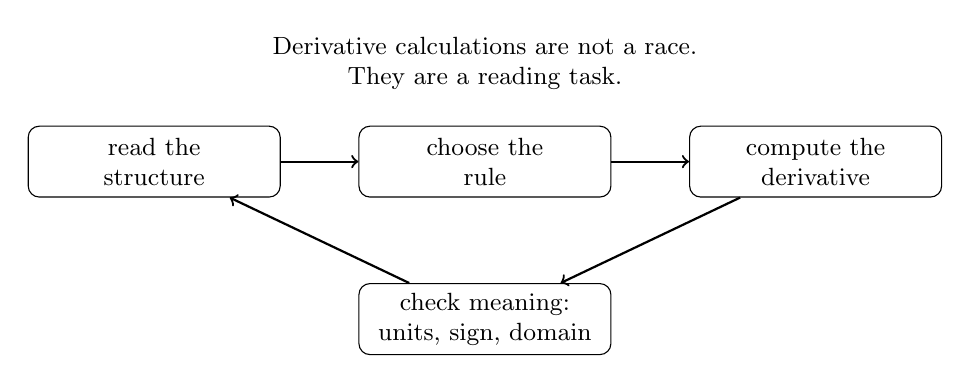
\begin{tikzpicture}[every node/.style={font=\small}, node distance=2.2cm]
  \node[draw, rounded corners, align=center, minimum width=3.2cm, minimum height=0.9cm] (structure) at (0,0)
  {read the\\ structure};

  \node[draw, rounded corners, align=center, minimum width=3.2cm, minimum height=0.9cm] (rule) at (4.2,0)
  {choose the\\ rule};

  \node[draw, rounded corners, align=center, minimum width=3.2cm, minimum height=0.9cm] (formula) at (8.4,0)
  {compute the\\ derivative};

  \node[draw, rounded corners, align=center, minimum width=3.2cm, minimum height=0.9cm] (meaning) at (4.2,-2.0)
  {check meaning:\\ units, sign, domain};

  \draw[->, thick] (structure) -- (rule);
  \draw[->, thick] (rule) -- (formula);
  \draw[->, thick] (formula) -- (meaning);
  \draw[->, thick] (meaning) -- (structure);

  \node[align=center] at (4.2,1.25)
  {Derivative calculations are not a race.\\
  They are a reading task.};
\end{tikzpicture}
\caption{A good derivative calculation reads the function first and checks the result afterward.}
\label{fig:chapter-5-derivative-workflow}
\end{figure}

\subsection{Derivative table}
\label{subsec:chapter-5-derivative-table}

The main elementary derivative formulas from this chapter are collected below.  Each formula is valid on intervals where the function is defined and differentiable.

\[
\boxed{
\begin{array}{c|c}
\textbf{function} & \textbf{derivative} \\ \hline
c & 0 \\[3pt]
x & 1 \\[3pt]
x^r & rx^{r-1} \\[3pt]
e^x & e^x \\[3pt]
a^x & (\ln a)a^x,\quad a>0 \\[3pt]
\ln x & \dfrac1x,\quad x>0 \\[8pt]
\ln|x| & \dfrac1x,\quad x\neq0 \\[8pt]
\sin x & \cos x \\[3pt]
\cos x & -\sin x \\[3pt]
\tan x & \sec^2x \\[3pt]
\sec x & \sec x\tan x \\[3pt]
\csc x & -\csc x\cot x \\[3pt]
\cot x & -\csc^2x \\[3pt]
\arcsin x & \dfrac1{\sqrt{1-x^2}} \\[8pt]
\arccos x & -\dfrac1{\sqrt{1-x^2}} \\[8pt]
\arctan x & \dfrac1{1+x^2} \\[8pt]
\sinh x & \cosh x \\[3pt]
\cosh x & \sinh x \\[3pt]
\tanh x & \operatorname{sech}^2x
\end{array}
}
\]

The table is only useful when paired with the rules:

\[
\boxed{
\begin{aligned}
(af+bg)'&=af'+bg',\\
(fg)'&=f'g+fg',\\
\left(\frac fg\right)'&=\frac{gf'-fg'}{g^2},\\
(f(g(x)))'&=f'(g(x))g'(x).
\end{aligned}
}
\]

Most real derivative calculations use both a table formula and a rule.

\subsection{Worked mixed examples}
\label{subsec:worked-mixed-derivative-examples}

\paragraph{Example.}
Differentiate

\[
F(x)=e^{-x}\cos(2x)+\ln(1+x^2).
\]

The first term is a product:

\[
e^{-x}\cos(2x).
\]

Differentiate each factor:

\[
\frac{d}{dx}e^{-x}=-e^{-x},
\]

and

\[
\frac{d}{dx}\cos(2x)=-2\sin(2x).
\]

So

\[
\frac{d}{dx}\left(e^{-x}\cos(2x)\right)
=
(-e^{-x})\cos(2x)+e^{-x}(-2\sin(2x)).
\]

Thus

\[
\frac{d}{dx}\left(e^{-x}\cos(2x)\right)
=
-e^{-x}\cos(2x)-2e^{-x}\sin(2x).
\]

The logarithmic term uses the chain rule:

\[
\frac{d}{dx}\ln(1+x^2)=\frac{2x}{1+x^2}.
\]

Therefore

\[
\boxed{
F'(x)
=
-e^{-x}\cos(2x)-2e^{-x}\sin(2x)
+
\frac{2x}{1+x^2}.
}
\]

We can factor the first two terms if desired:

\[
F'(x)
=
-e^{-x}\bigl(\cos(2x)+2\sin(2x)\bigr)
+
\frac{2x}{1+x^2}.
\]

\paragraph{Example.}
Differentiate

\[
y=(x^2+1)^{\sin x}.
\]

This function has a variable exponent.  Since the base is always positive,

\[
x^2+1>0,
\]

logarithmic differentiation is safe.

Take natural logarithms:

\[
\ln y=\sin x\ln(x^2+1).
\]

Differentiate both sides:

\[
\frac{y'}{y}
=
\cos x\ln(x^2+1)
+
\sin x\cdot\frac{2x}{x^2+1}.
\]

Multiply by \(y\):

\[
y'
=
y\left(
\cos x\ln(x^2+1)
+
\frac{2x\sin x}{x^2+1}
\right).
\]

Substitute back

\[
y=(x^2+1)^{\sin x}.
\]

Thus

\[
\boxed{
y'
=
(x^2+1)^{\sin x}
\left(
\cos x\ln(x^2+1)
+
\frac{2x\sin x}{x^2+1}
\right).
}
\]

This example uses several ideas at once: logarithms, product rule, chain rule, and the fact that \(x^2+1\) is positive.

\paragraph{Example.}
Find \(dy/dx\) if

\[
x^2y+\sin y=e^x.
\]

Here \(y\) is treated as a function of \(x\).  Differentiate both sides with respect to \(x\).

For \(x^2y\), use the product rule:

\[
\frac{d}{dx}(x^2y)=2xy+x^2y'.
\]

For \(\sin y\), use the chain rule:

\[
\frac{d}{dx}\sin y=\cos y\,y'.
\]

For \(e^x\),

\[
\frac{d}{dx}e^x=e^x.
\]

Therefore

\[
2xy+x^2y'+\cos y\,y'=e^x.
\]

Collect the \(y'\)-terms:

\[
(x^2+\cos y)y'=e^x-2xy.
\]

So

\[
\boxed{
\frac{dy}{dx}
=
\frac{e^x-2xy}{x^2+\cos y}.
}
\]

The denominator warns us: if

\[
x^2+\cos y=0,
\]

then this equation does not determine a finite value of \(dy/dx\).  The algebra may be pointing to a vertical tangent or to a place where the curve is not a single differentiable branch \(y(x)\).

\subsection{Skills: mixed derivative calculations}
\label{subsec:mixed-derivative-calculations}

Differentiate each function.  State domain restrictions when they affect the derivative.

\begin{enumerate}
\item
\[
f(x)=(4x^3-2x+7)^5.
\]

\item
\[
f(x)=x^2e^{-3x}.
\]

\item
\[
f(x)=\frac{\sin x}{1+\cos x}.
\]

\item
\[
f(x)=\ln|x^2-5x+6|.
\]

\item
\[
f(x)=\arctan(e^x).
\]

\item
\[
f(x)=\sqrt{1+\sin^2x}.
\]

\item
\[
f(x)=2^{x^2}.
\]

\item
\[
f(x)=\sin(\ln x).
\]

\item
\[
f(x)=x^{\sqrt3}\cos x,
\qquad x>0.
\]

\item
\[
f(x)=(\ln x)^3\sqrt{x},
\qquad x>0.
\]

\item
\[
f(x)=\frac{e^x}{1+x^2}.
\]

\item
\[
f(x)=\arcsin(2x).
\]

\item
\[
f(x)=x^x,
\qquad x>0.
\]

\item
\[
f(x)=(\cos x)^x
\]

on an interval where \(\cos x>0\).

\item
\[
f(x)=\tanh(5x).
\]

\item
\[
f(x)=\sinh(x^2)\cosh x.
\]

\item
\[
f(x)=e^{\sin x}\ln(1+x^2).
\]

\item
\[
f(x)=\frac{\arctan x}{x},
\qquad x\neq0.
\]

\item
\[
f(x)=\ln(\sec x+\tan x)
\]

on an interval where the logarithm is defined.

\item
\[
f(x)=\sqrt[3]{1+x^4}.
\]

\item
\[
f(x)=\frac{\sin(x^2)}{e^x}.
\]

\item
\[
f(x)=\cos(\sqrt{x}),
\qquad x>0.
\]

\item
\[
f(x)=\arctan\left(\frac{1}{x}\right),
\qquad x\neq0.
\]

\item
\[
f(x)=\frac{x^2+1}{\sqrt{x^2-1}}.
\]

\item
\[
f(x)=\ln\left(\frac{x^2+1}{x-1}\right),
\qquad x>1.
\]

\item
\[
f(x)=(1+\sin x)^{4}.
\]

\item
\[
f(x)=e^{x\cos x}.
\]

\item
\[
f(x)=\arccos(1-x^2).
\]

\item
\[
f(x)=\frac{\sinh x}{1+\cosh x}.
\]

\item
\[
f(x)=\left(\frac{x+1}{x-1}\right)^x
\]

on an interval where the base is positive.
\end{enumerate}

\subsection{Implicit differentiation practice}
\label{subsec:implicit-differentiation-practice-chapter-5}

Find \(dy/dx\).  Then find the tangent slope at the given point when a point is provided.

\begin{enumerate}
\item
\[
x^2+y^2=10.
\]

\item
\[
x^2+xy+y^2=7.
\]

\item
\[
y^3+xy=10,
\qquad (1,2).
\]

\item
\[
x^2y+\sin y=e^x.
\]

\item
\[
e^{xy}+y^2=x+2.
\]

\item
\[
\ln(x+y)=xy.
\]

\item
\[
\sin(xy)=x-y.
\]

\item
\[
x^3+y^3=6xy.
\]

\item
Find \(y''\) for the circle
\[
x^2+y^2=25.
\]

\item
For
\[
x^2+y^2=25,
\]
find all points on the circle where the tangent line is horizontal.  Then find all points where the tangent line is vertical.
\end{enumerate}

\subsection{Concept check}
\label{subsec:chapter-5-concept-check}

Answer each question in complete sentences.

\begin{enumerate}
\item Why does the product rule have two terms?

\item In the chain rule
\[
(f(g(x)))'=f'(g(x))g'(x),
\]
why is \(f'\) evaluated at \(g(x)\) instead of at \(x\)?

\item Why must angles be measured in radians for
\[
(\sin x)'=\cos x
\]
to be true without an extra constant?

\item Why does implicit differentiation require the chain rule?

\item In the inverse derivative formula
\[
(f^{-1})'(b)=\frac1{f'(a)},
\qquad b=f(a),
\]
why must the derivative of \(f\) be evaluated at \(a\), not at \(b\)?

\item Give an example of a function that has an inverse, but whose inverse is not differentiable at one point.

\item Explain why logarithmic differentiation is useful for
\[
y=x^x.
\]

\item The formulas
\[
(\sinh x)'=\cosh x
\qquad\text{and}\qquad
(\cosh x)'=\sinh x
\]
look similar to the sine and cosine formulas.  Where does the sign difference appear?
\end{enumerate}

\subsection{True or false}
\label{subsec:chapter-5-true-false}

Decide whether each statement is true or false.  If it is false, give a correction or a counterexample.

\begin{enumerate}
\item
\[
(fg)'=f'g'
\]
for all differentiable functions \(f\) and \(g\).

\item
\[
(f+g)'=f'+g'
\]
for all differentiable functions \(f\) and \(g\).

\item
\[
\frac{d}{dx}\sin(x^2)=2x\cos(x^2).
\]

\item
\[
\frac{d}{dx}(\sin x)^2=2x\cos(x^2).
\]

\item
\[
\frac{d}{dx}\ln|x|=\frac1x
\]
for \(x\neq0\).

\item
\[
\frac{d}{dx}a^x=xa^{x-1}
\]
for every positive constant \(a\).

\item
\[
\frac{d}{dx}x^a=ax^{a-1}
\]
for a fixed real number \(a\), at least for \(x>0\).

\item If \(f'(a)=0\), then \(f\) cannot have an inverse.

\item If \(f\) has an inverse and \(f'(a)=0\), then the formula
\[
(f^{-1})'(f(a))=\frac1{f'(a)}
\]
cannot be used.

\item The derivative of \(\arctan x\) exists for every real \(x\).
\end{enumerate}

\subsection{Proof practice}
\label{subsec:chapter-5-proof-practice}

These problems ask you to justify the rules, not only use them.

\begin{enumerate}
\item \textbf{Product rule from the definition.}
Suppose \(f\) and \(g\) are differentiable at \(x\).  Starting from

\[
\frac{f(x+h)g(x+h)-f(x)g(x)}{h},
\]

add and subtract

\[
f(x+h)g(x)
\]

in the numerator.  Use this to prove

\[
(fg)'(x)=f'(x)g(x)+f(x)g'(x).
\]

\item \textbf{Reciprocal rule from the product rule.}
Let

\[
q(x)=\frac1{g(x)},
\]

where \(g(x)\neq0\).  Since

\[
g(x)q(x)=1,
\]

differentiate both sides and solve for \(q'(x)\).  Prove

\[
\left(\frac1g\right)'=-\frac{g'}{g^2}.
\]

\item \textbf{Quotient rule from product and reciprocal rules.}
Write

\[
\frac{f}{g}=f\cdot\frac1g.
\]

Use the product rule and reciprocal rule to prove

\[
\left(\frac fg\right)'=\frac{gf'-fg'}{g^2}.
\]

\item \textbf{Chain rule using local linearity.}
Suppose

\[
u=g(x),
\qquad
y=f(u).
\]

Use the approximations

\[
g(x+h)=g(x)+g'(x)h+\text{small error}
\]

and

\[
f(u+k)=f(u)+f'(u)k+\text{small error}
\]

to explain why

\[
\frac{d}{dx}f(g(x))=f'(g(x))g'(x).
\]

\item \textbf{Inverse derivative formula.}
Let \(g=f^{-1}\).  Starting from

\[
f(g(x))=x,
\]

differentiate both sides using the chain rule.  Solve for \(g'(x)\) and obtain

\[
(f^{-1})'(x)=\frac1{f'(f^{-1}(x))}.
\]

What condition is needed to divide?

\item \textbf{Derivative of \(\ln x\) from the inverse rule.}
Use the fact that \(\ln x\) is the inverse of \(e^x\) to prove

\[
\frac{d}{dx}\ln x=\frac1x.
\]

\item \textbf{General power rule.}
For \(x>0\), let

\[
y=x^r,
\]

where \(r\) is a fixed real number.  Take logarithms and differentiate implicitly to prove

\[
\frac{d}{dx}x^r=rx^{r-1}.
\]
\end{enumerate}

\subsection{Project: derivative formulas from numerical experiments}
\label{subsec:project-derivative-formulas-numerical-experiments}

A derivative is a limit.  Numerical experiments can suggest what the limit is before we prove it.

For a small positive number \(h\), define the symmetric difference quotient

\[
D_h f(a)=\frac{f(a+h)-f(a-h)}{2h}.
\]

This often gives a better numerical estimate of \(f'(a)\) than the one-sided quotient

\[
\frac{f(a+h)-f(a)}{h}.
\]

The goal of this project is to rediscover several derivative formulas from data.

\paragraph{Step 1: choose step sizes.}
Use

\[
h=10^{-1},\ 10^{-2},\ 10^{-3},\ 10^{-4},\ 10^{-5},\ 10^{-6}.
\]

For each function and each point \(a\), compute

\[
D_h f(a).
\]

Organize your results in a table.

\[
\begin{array}{c|cccccc}
h & 10^{-1} & 10^{-2} & 10^{-3} & 10^{-4} & 10^{-5} & 10^{-6} \\ \hline
D_h f(a) & & & & & &
\end{array}
\]

\paragraph{Step 2: test powers.}
Use

\[
f(x)=x^2,\qquad f(x)=x^3,\qquad f(x)=\sqrt{x}.
\]

Test at

\[
a=1,\quad a=2,\quad a=4.
\]

Use the numerical estimates to guess the formulas for

\[
(x^2)',\qquad
(x^3)',\qquad
(\sqrt{x})'.
\]

Compare your guesses with the power rule.

\paragraph{Step 3: test trigonometric functions.}
Use radians.  Compute numerical derivatives for

\[
f(x)=\sin x
\qquad\text{and}\qquad
f(x)=\cos x
\]

at

\[
a=0,\quad \frac{\pi}{6},\quad \frac{\pi}{4},\quad \frac{\pi}{3},\quad \frac{\pi}{2}.
\]

Compare the numerical derivative of \(\sin x\) with \(\cos x\).  Compare the numerical derivative of \(\cos x\) with \(-\sin x\).

Then repeat the experiment using degrees by defining

\[
S(x)=\sin(x^\circ)=\sin\left(\frac{\pi x}{180}\right).
\]

Estimate \(S'(30)\).  Explain why the extra factor

\[
\frac{\pi}{180}
\]

appears.

\paragraph{Step 4: test exponentials.}
For

\[
f(x)=a^x,
\]

the derivative should be proportional to \(a^x\).  Estimate

\[
\frac{D_h f(0)}{f(0)}
\]

for

\[
a=2,\quad a=3,\quad a=10.
\]

Since \(f(0)=1\), this is just the estimated slope at \(0\).  Compare the results with

\[
\ln2,\qquad \ln3,\qquad \ln10.
\]

Now test

\[
f(x)=e^x.
\]

Estimate \(D_h f(a)\) at

\[
a=-1,\quad 0,\quad 1,\quad 2.
\]

Compare with \(e^a\).

\paragraph{Step 5: test logarithms.}
Use

\[
f(x)=\ln x.
\]

Estimate \(f'(a)\) at

\[
a=1,\quad 2,\quad 5,\quad 10.
\]

Compare with

\[
\frac1a.
\]

\paragraph{Step 6: watch roundoff.}
Try step sizes smaller than \(10^{-6}\), such as

\[
10^{-8},\quad 10^{-10},\quad 10^{-12}.
\]

Do the estimates always improve?  Explain what you see.

Your report should answer three questions:

\[
\begin{array}{l}
\text{1. Which derivative formulas did your data suggest?}\\
\text{2. Where did the numerical evidence become unreliable?}\\
\text{3. Why is a proof still needed after a convincing table of values?}
\end{array}
\]

\subsection{Discovery problems}
\label{subsec:chapter-5-discovery-problems}

\begin{enumerate}
\item \textbf{A hidden product rule.}
Let

\[
A(x)=(x+1)(x+2)(x+3).
\]

Differentiate \(A(x)\) in two ways:

\[
\text{first by expanding,}
\]

and

\[
\text{then by applying the product rule twice.}
\]

Show that the two answers agree.

\item \textbf{A pattern for logarithmic derivatives.}
Let

\[
P(x)=(x-a_1)(x-a_2)\cdots(x-a_n).
\]

Assume all factors are nonzero.  Take logarithms and differentiate to show

\[
\frac{P'(x)}{P(x)}
=
\frac1{x-a_1}+\frac1{x-a_2}+\cdots+\frac1{x-a_n}.
\]

This formula is useful because it turns a product into a sum.

\item \textbf{A tangent to an inverse without finding the inverse.}
Let

\[
f(x)=x^5+x.
\]

Show that \(f\) is increasing.  Find

\[
(f^{-1})'(2)
\]

without solving for \(f^{-1}(x)\).

\item \textbf{Two functions with the same value but different local behavior.}
Find two differentiable functions \(f\) and \(g\) such that

\[
f(0)=g(0)
\]

but

\[
f'(0)\neq g'(0).
\]

Explain in words what this means about their graphs near \(0\).

\item \textbf{Two functions with the same derivative at one point but different graphs.}
Find two differentiable functions \(f\) and \(g\) such that

\[
f'(0)=g'(0)
\]

but the graphs do not look the same near \(0\).

\item \textbf{A derivative that simplifies unexpectedly.}
Differentiate

\[
f(x)=\frac{1-\cos x}{\sin x}
\]

where it is defined.  Then use trigonometric identities to simplify the derivative.

\item \textbf{A logarithmic identity through derivatives.}
Let

\[
F(x)=\ln(\sec x+\tan x).
\]

Differentiate \(F\).  On intervals where the functions are defined, show that

\[
F'(x)=\sec x.
\]

This identity will become useful when we integrate \(\sec x\).

\item \textbf{A hyperbolic simplification.}
Differentiate

\[
f(x)=\ln(\cosh x).
\]

Express the answer using \(\tanh x\).

\item \textbf{A variable base and variable exponent.}
For \(x>0\), differentiate

\[
f(x)=x^{\ln x}.
\]

Hint: take logarithms first.

\item \textbf{A curve with no solved formula.}
The equation

\[
x^3+y^3=6xy
\]

defines a curve called the folium of Descartes.  Use implicit differentiation to find \(dy/dx\).  Then find the slope at

\[
(3,3).
\]
\end{enumerate}

\subsection{Where the chapter points next}
\label{subsec:chapter-5-hook-shape}

A derivative is more than a number to compute.  It is information about shape.

For example, consider

\[
f(x)=x^3-3x.
\]

Its derivative is

\[
f'(x)=3x^2-3=3(x-1)(x+1).
\]

The derivative is positive when

\[
x<-1
\]

and when

\[
x>1.
\]

It is negative when

\[
-1<x<1.
\]

The graph rises, then falls, then rises again.
\begin{figure}[h]
\centering
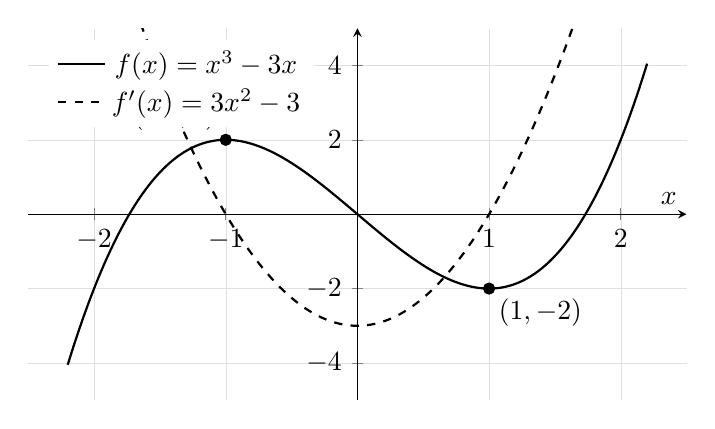
\begin{tikzpicture}
\begin{axis}[
    width=0.82\textwidth,
    height=0.52\textwidth,
    xmin=-2.5, xmax=2.5,
    ymin=-5, ymax=5,
    axis lines=middle,
    xlabel={\(x\)},
    ylabel={},
    xtick={-2,-1,0,1,2},
    ytick={-4,-2,0,2,4},
    grid=both,
    grid style={line width=.1pt, draw=gray!25},
    legend style={draw=none, at={(0.03,0.97)}, anchor=north west}
]
\addplot[thick, domain=-2.2:2.2, samples=200] {x^3-3*x};
\addlegendentry{\(f(x)=x^3-3x\)}
\addplot[thick, dashed, domain=-2.2:2.2, samples=200] {3*x^2-3};
\addlegendentry{\(f'(x)=3x^2-3\)}
\addplot[only marks, mark=*] coordinates {(-1,2) (1,-2)};
\node[anchor=south east] at (axis cs:-1,2) {\((-1,2)\)};
\node[anchor=north west] at (axis cs:1,-2) {\((1,-2)\)};
\end{axis}
\end{tikzpicture}
\caption{The derivative gives information about the shape of the original graph.}
\label{fig:chapter-5-hook-derivative-shape}
\end{figure}

At

\[
x=-1
\qquad\text{and}\qquad
x=1,
\]

the derivative is \(0\).  The graph has horizontal tangents there.  One is a high point nearby; the other is a low point nearby.

That observation opens the next part of the book.

Derivatives compute slopes.  But slopes tell us when a function rises, when it falls, where it turns, and where it bends.  The next chapter asks how much of a graph we can understand from its derivative.